
\section{Results}
\label{sec:results}

To demonstrate the effectiveness of the iterative algorithm for MFA computation, we devised a series of analytical closed form functionals and utilized real-world scientific datasets in both 2- and 3-dimensions obtained from high-fidelity simulations. All runs shown in this section were performed using the Python drivers written specifically for this work using the \texttt{DIY} domain decomposition infrastructure.

%A brief description of the problem cases that are used as test datasets is given below.
%
%\begin{enumerate}
%	\item Synthetic data: sinc($x$)=$\frac{sin(x)}{x}$ functional on $\Omega \in [-4, 4]$
%	\begin{itemize}
%		\item \textbf{Symmetric \dimension{1}:} Q(x) = 100(sinc($x$-1) + sinc($x$+1))
%		\item \textbf{Asymmetric \dimension{1}:} Q(x) = sinc($x$) + sinc(2$x$-1) + sinc(3$x$+1.5), 
%		% z = scale * ( np.sinc((X+1)**2 + (Y-1)**2) + np.sinc(((X-1)**2 + (Y+1)**2)) )
%		\item \textbf{Analytical 2d:} Q(x,y) = sinc($(x+1)^2+(y-1)^2$) + sinc($(x-1)^2+(y+1)^2$)
%	\end{itemize}
%%	\item Nek5000: A 3-D dataset from CFD simulation with velocity magnitude as the solution profile
%	\item S3D: A 3-D turbulent combustion dataset generated by an S3D simulation \cite{chen-s3d-2009} of fuel jet combustion in the presence of an external cross-flow. 
%	\item CESM: A 2-D Community Atmosphere Model climate model dataset on a sphere with 3600x1800 resolution
%\end{enumerate}


\subsection{\dimension{1} Results}\label{sec:results-1d}

In this section, detailed analysis on the convergence and accuracy of various MFA continuity recovery approaches are presented. 
%\begin{itemize}
%	\item Use the first two problems to measure convergence in parallel as number of domains increase
%	\item Talk about adaptivity and resolution of data even for highly varying problem data.
%\end{itemize}

\subsubsection{Comparison of Clamped vs Floating Boundary Knots}

To demonstrate the choice of using floating knots vs the low-order ($C^0$) continuous clamped knots at subdomain boundaries, we choose an analytical closed form reference solution of the form:

\begin{equation}
	F(x) = sinc(x) + sinc(2x-1) + sinc(3x+1.5), \forall x \in \Omega=[-4, 4]
	\label{eqn:1d-asymmetric-sinc}
\end{equation}

The reference solution $F(x)$, the results from the clamped knots, and floating knots with and without augmented overlap regions $\delta=p$ are shown in \fig{fig:comparison-clamped-floating}. The figures show the recovered solutions and the corresponding decoded error from MFA evaluation for a $\mathcal{N}=2$ and $p=3$ case. It is evident that the net error profile in the fully clamped subdivision in this example shows lower error as compared to the floating knot experiments. However, it is imperative to note that the former only shows $C^0$ regularity, while the floating knots fully recover high-order continuity at subdomain interfaces. Moreover, the use of augmented overlap regions ($\delta=3$) produce error profiles that resemble a single subdomain error profile in the domain, which is one of the key metrics of interest. These behaviors and conclusions extend to multi-dimensional setting as well.

\begin{figure}[htbp]
	\centering
	\subfloat[Input analytical \dimension{1} solution profile\label{fig:1d-reference}]{%
		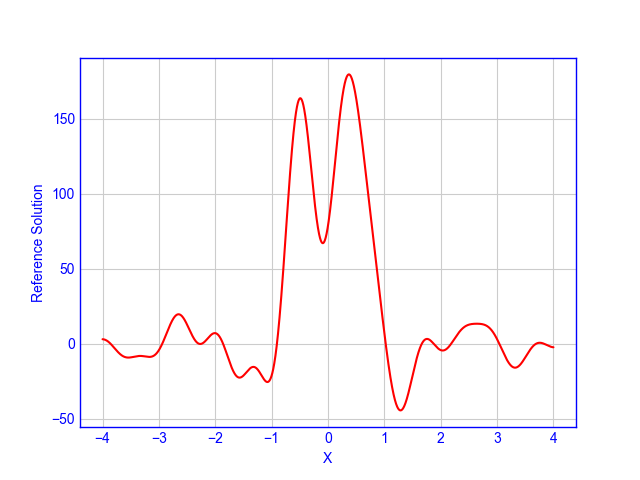
\includegraphics[width=0.44\textwidth]{figures/1d-reference-solution}}
	\quad \quad
	\subfloat[Clamped $C^0$ continuous decoded solution\label{fig:1d-clamped}]{%
		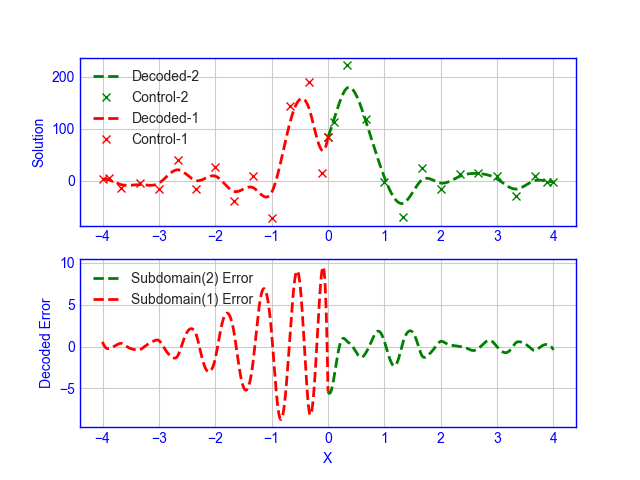
\includegraphics[width=0.44\linewidth]{figures/1d-clamped-2subd}}
	\\
	\subfloat[Floating knots at $\Omega_{1,2}$ recovering $C^{p-1}$ continuity\label{fig:1d-unclamped}]{%
		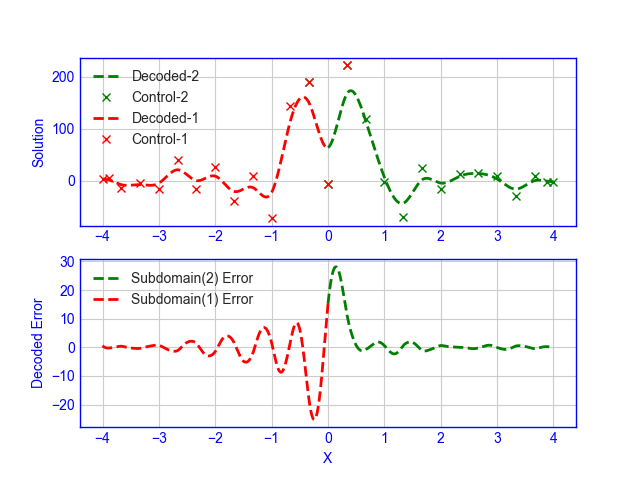
\includegraphics[width=0.44\linewidth]{figures/1d-unclamped-2subd}}
	\quad \quad
	\subfloat[Floating knots at $\Omega_{1,2}$ with $\left| \delta \right|=3$ \label{fig:1d-unclamped-aug}]{%
		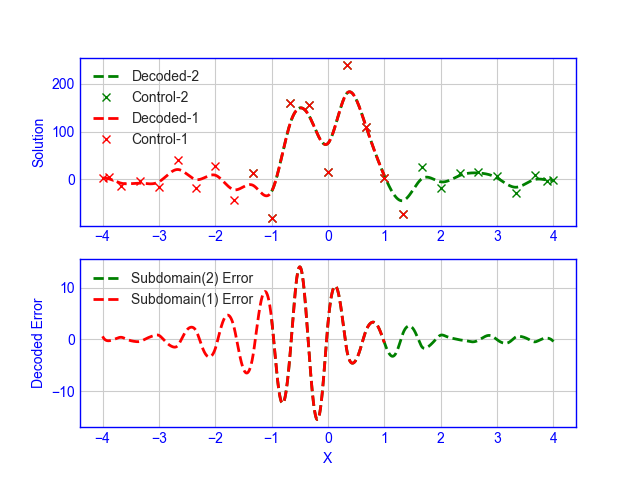
\includegraphics[width=0.44\linewidth]{figures/1d-unclamped-aug-2subd}}
	\caption{\dimension{1} analytical sinc dataset with 10000 input points with $\mathcal{N}=2$ and $p=3$}
	\label{fig:comparison-clamped-floating}
\end{figure}


%\comment{Discuss that the error in clamped solution are lower but only $C^0$, while in the floating version, we get $C^p$}

%\subsubsection{Error Convergence and Continuity Verification}

To further demonstrate the continuity recovery behavior, we plot the error profile $\vec{E}$ for these approaches in \fig{fig:1d-error-comparison}, zoomed in around the interface $\Omega_{1,2}$. The unconstrained and decoupled LSQ solution procedure in the top shows that the reconstructed solution is discontinuous at the interface, as expected. Using the fully clamped approach that yields lower overall absolute error showcases only $C^0$ continuity at the interface, which may or not be sufficient depending on the use case utilizing the MFA representation. Finally, the bottom plot shows the smooth error profile from using the floating knots at the interface with full recovery of high-order continuity. We again emphasize that one could recover $C^0$ to $C^{p-1}$ continuity with this approach by choosing to use floating knots vs varying number of repeated knots at the interface.

%The solution profile, along with control point locations from the adaptive computations are shown in \fig{fig:sinc-adaptive-a}. We utilized the residual definition shown in \eqt{eq:nonlinear-residuals} to ensure $C_2$ continuity (with $p=3$) to be satisfied along all internal subdomain interfaces. The \fig{fig:sinc-adaptive-b} and \fig{fig:sinc-adaptive-c} present the zoomed in reconstruction of the approximation near the interface between $\Omega_2$ and $\Omega_3$ before, and after the ASM iterations are converged. The initially discontinuous solutions from independent, adaptive, unconstrained subdomain solves resulting in \fig{fig:sinc-adaptive-b} are then iteratively converged to satisfy all constraints after 3 RAS iterations, with nearest neighbor exchange of control point data at the interfaces to recover $C_2$ continuity.

\begin{figure}[htbp]
	\centering
	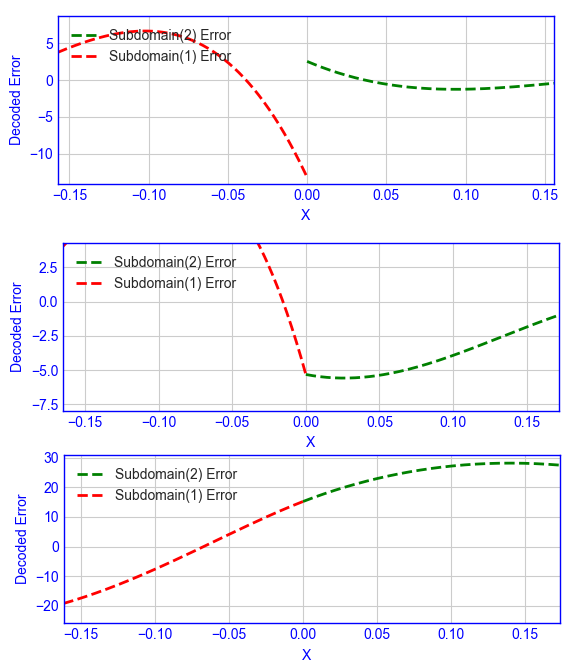
\includegraphics[width=0.44\textwidth]{figures/1d-error-comparison}
	\caption{Zoomed error plots at interface $\Omega_{1,2}$ for \dimension{1} analytical dataset with $10^4$ input points, $\mathcal{N}=2$ and $p=3$.  Top: unconstrained and decoupled subdomain profile (discontinuous). Middle: clamped interface knots. Bottom: floating interface knots.}
	\label{fig:1d-error-comparison}
\end{figure}

%\subsubsection{Subdomain Solver Performance}
%
%Compare LCLSQ - Encoded nonlinear and Decoded nonlinear

\subsubsection{Error Convergence and Overlap Experiments}

To determine the effect of using augmented or overlapped knot span regions ($\delta$) as the number of subdomains $\mathcal{N}$ are increased, we use a fully symmetric double-sinc function as shown below in \eqt{eqn:1d-symmetric-sinc} on a single subdomain as the reference solution as shown in \fig{fig:error-1d-a}, and with $\mathcal{N}=5$ for different values of augmented spans ($\left| \delta \right|=0$ and $\left| \delta \right|=3$).


\begin{equation}
	F(x) = sinc(x+1) + sinc(x-1), \forall x \in \Omega=[-4, 4]
	\label{eqn:1d-symmetric-sinc}
\end{equation}


\begin{figure}[htbp]
	\centering
	\subfloat[A double sinc profile in \dimension{1}\label{fig:error-1d-a}]{%
		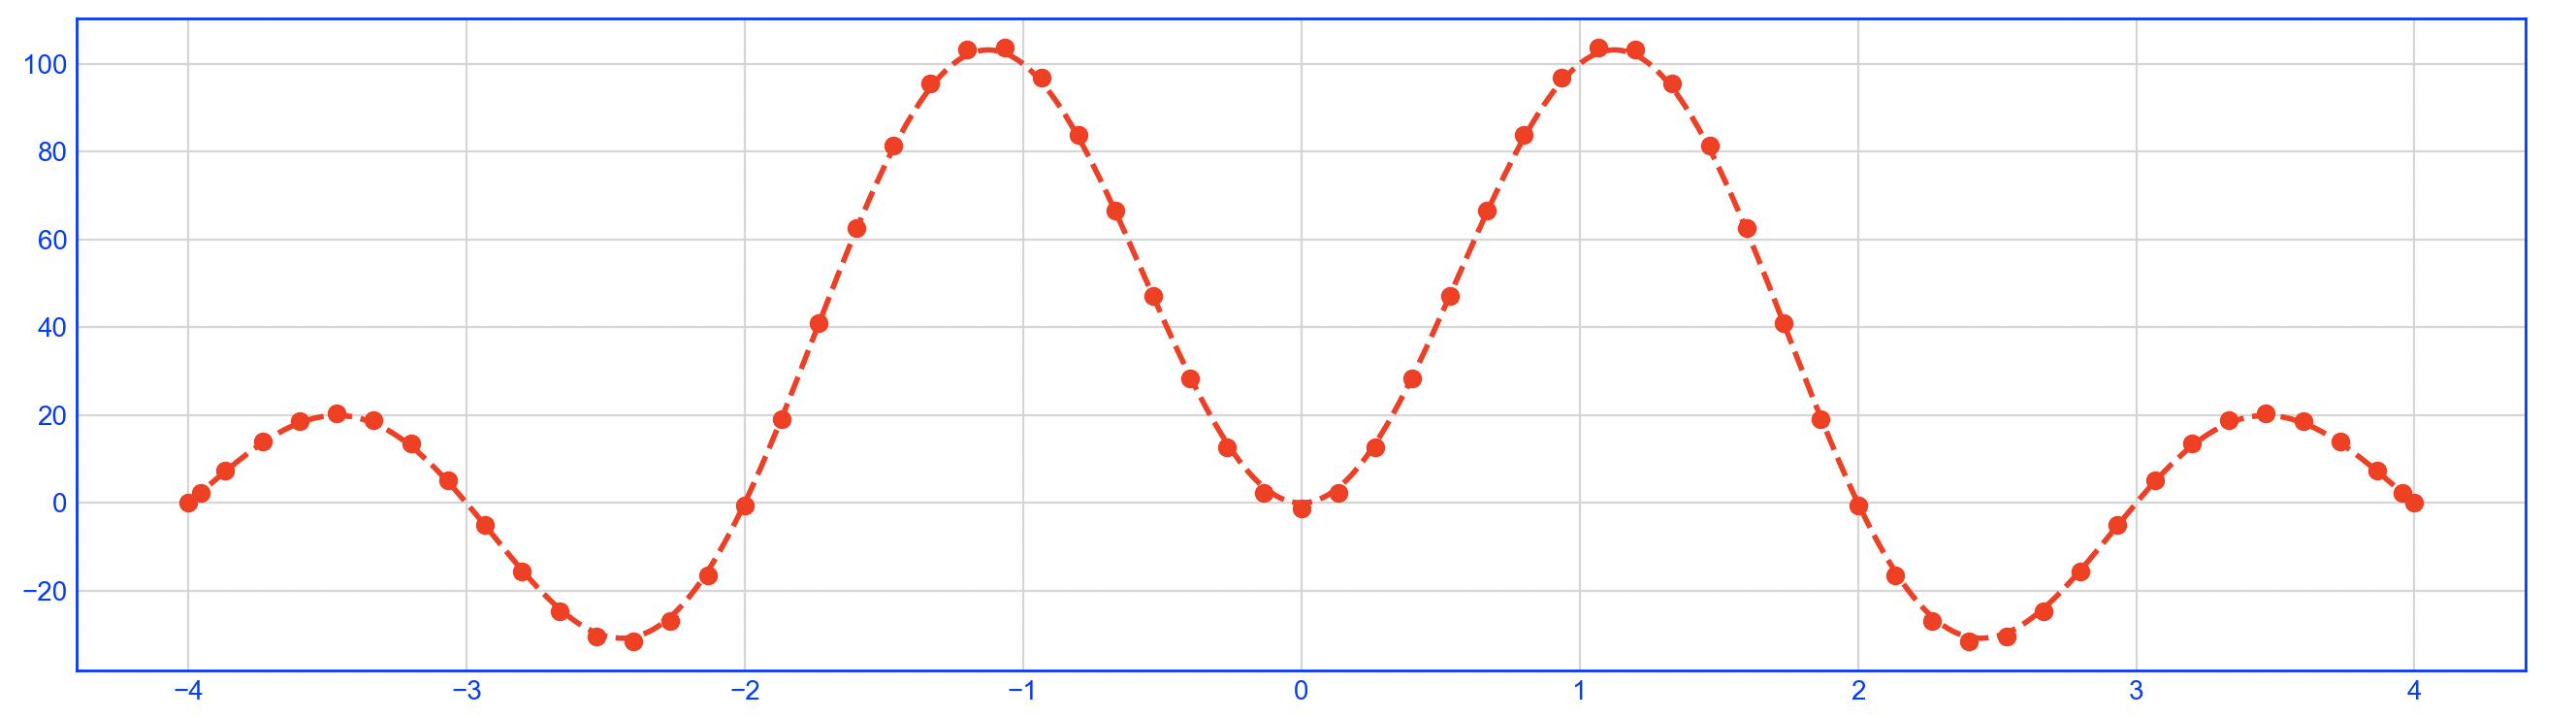
\includegraphics[width=0.5\textwidth]{figures/sol-subd1-cpts63-d3-g0.png}}
	\hfill
	\subfloat[Error profile for $\mathcal{N}=1$ and $p=3$\label{fig:error-1d-b}]{%
		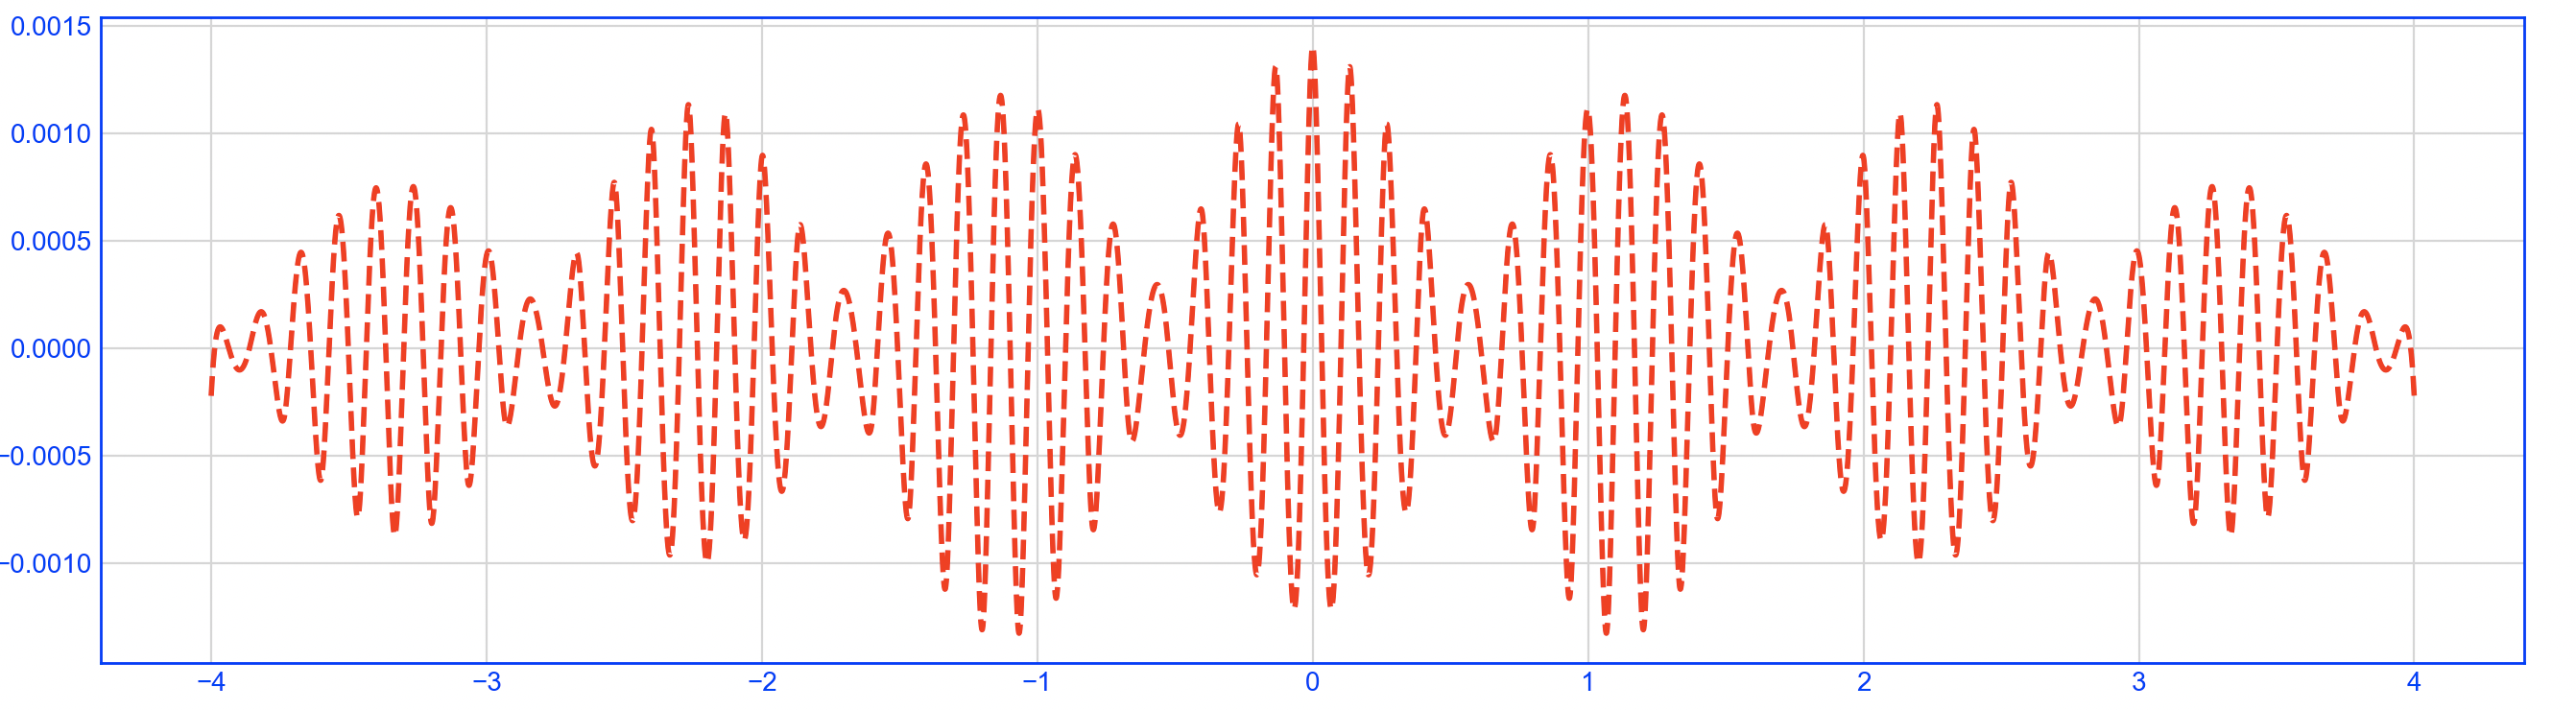
\includegraphics[width=0.5\textwidth]{figures/subd1-cpts63-d3-g0.png}}
	\\
	\subfloat[Error profile for $\mathcal{N}=5$, $p=3$ and $\left| \delta \right|=0$\label{fig:error-1d-c}]{%
		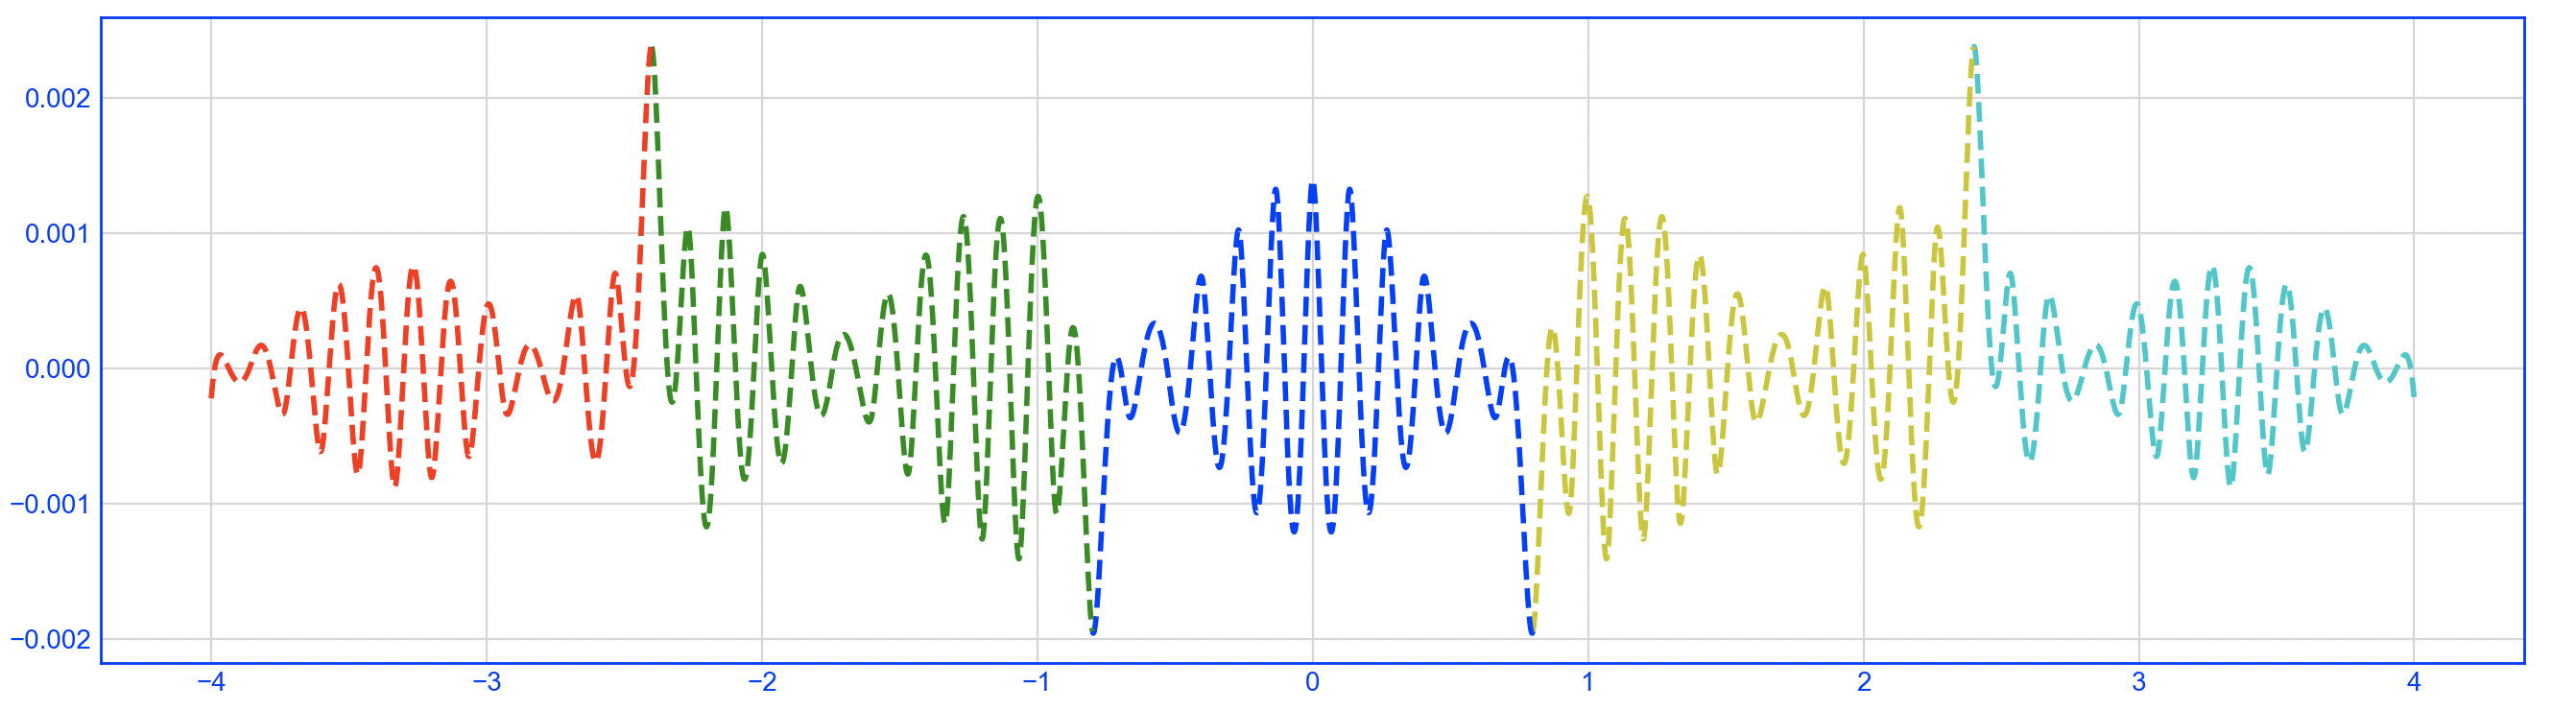
\includegraphics[width=0.5\textwidth]{figures/subd5-cpts15-d3-g0.png}}
	\hfill
	\subfloat[Error profile for $\mathcal{N}=5$, $p=3$ and $\left| \delta \right|=p$\label{fig:error-1d-d}]{%
	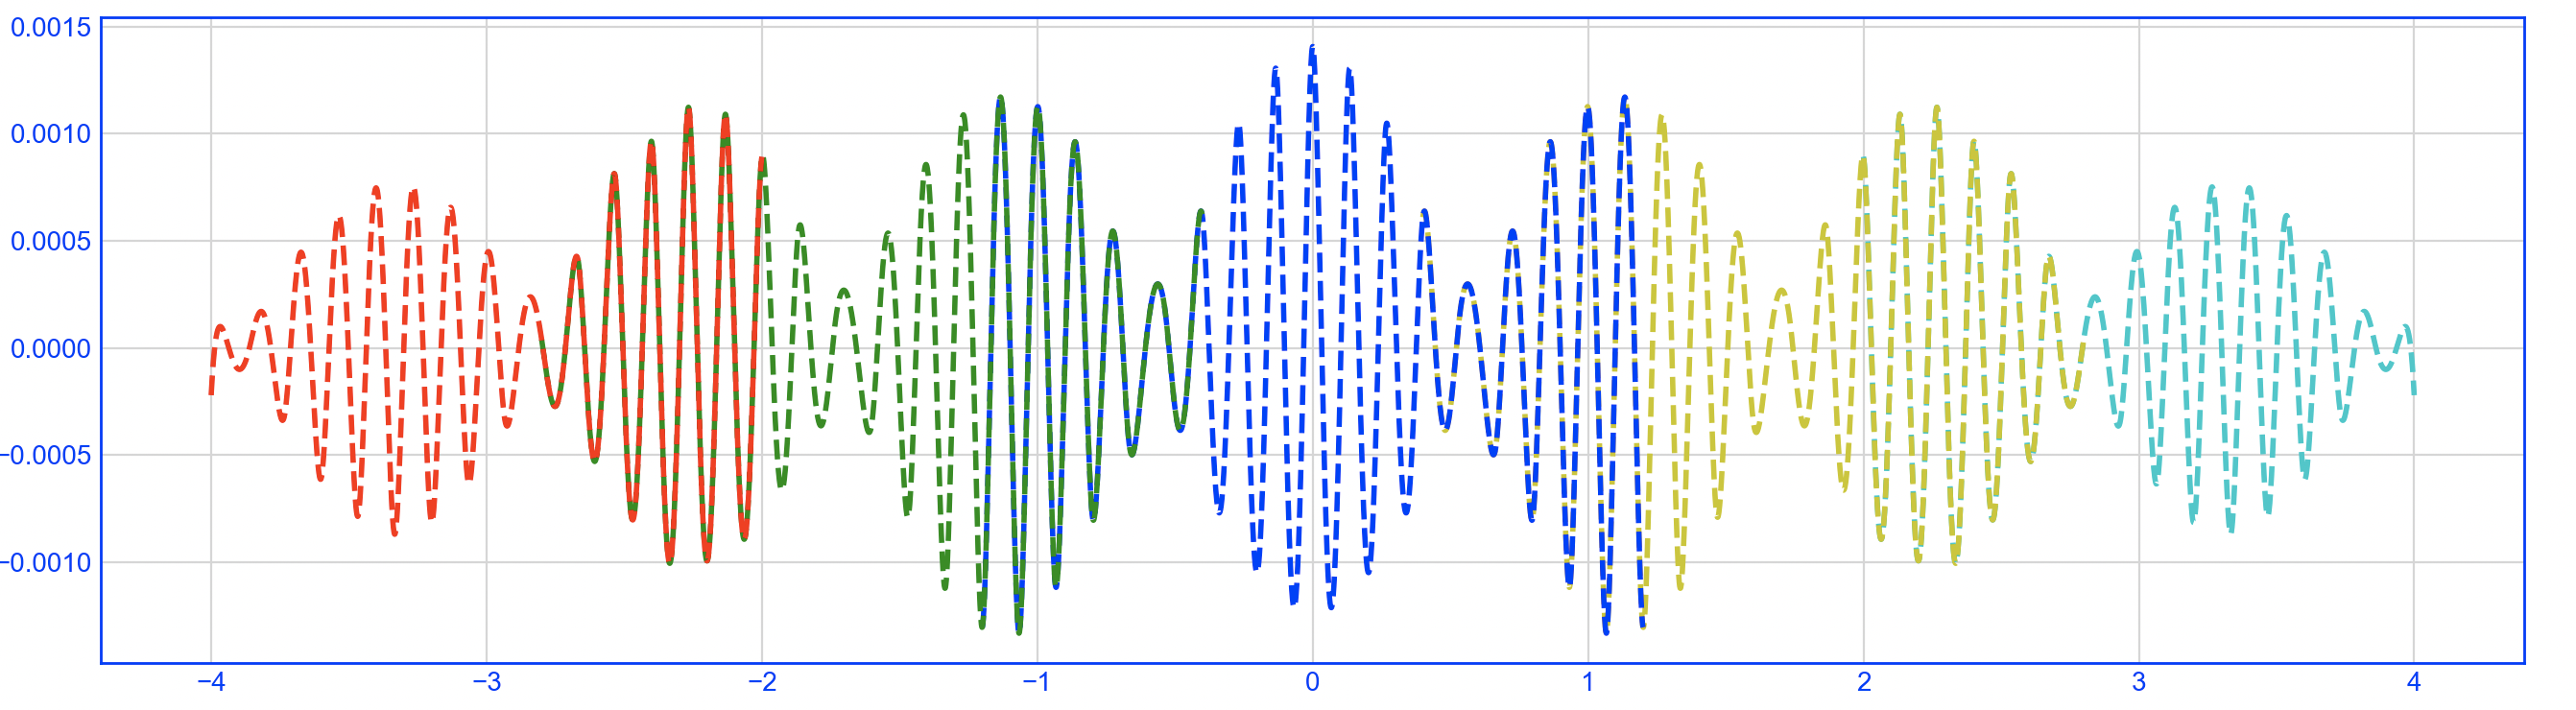
\includegraphics[width=0.5\textwidth]{figures/subd5-cpts15-d3-g3.png}}
	\caption{Demonstration of error convergence, and effect of the overlapping spans to minimize numerical artifacts}
	\label{fig:error-1d}
\end{figure}

It is evident from \fig{fig:error-1d-c} that when there is no augmented knot spans used in a multi-subdomain solver, the decoding of data at subdomain boundaries are influenced by contributions from both adjacent domain DoFs, which are enforced to be $C^{p-1}$ continuous by the constrained minimization solver. However, as we increase the number of overlap regions in terms of both the underlying data and the local bases support spans, the error profiles as shown in \fig{fig:error-1d-d} approaches the reference profile (with $\mathcal{N}=1$) shown in \fig{fig:error-1d-b}. Heuristically, for many of the problems tested, using $\left| \delta \right|=p$ provides optimal convergence as number of subdomains increase, even though increasing this parameter to $\left| \delta \right| =2p$ or higher will in general always improve the numerical accuracy at the cost of higher communication costs between neighboring subdomains.

%\comment{Might be worthwhile to evaluate (first) derivatives and show continuity there as well}


\subsection{Multi-dimensional Problem Cases}

In this section, we present some results from applying parallel MFA for multidimensional problem cases.

\subsubsection{2D Problem}

A \dimension{3} vector field representing the numerical results of a large-eddy simulation of Navier-Stokes equations for the MAX experiment \cite{merzari2010numerical} is representative of turbulent mixing and thermal striping that occur in the upper plenum of liquid sodium fast reactors. The data, generated by the Nek5000 solver \cite{deville2002}, have been resampled from their original topology onto a $200 \times 200 \times 200$ regular grid, and the magnitude of the velocity vector is associated with each \dimension{3} domain point \cite{peterka-mfa}.
%
Out of this dataset, a 2D slice (with $\left| \Omega \right|=200\times 200$) along the midplane in axial direction is used for our first study here. The reference solution and the converged, reconstructed solution with $\mathcal{N}=5 \times 5=25$ subdomains with $p=6$ and $\left| \delta \right|=2p$ is shown in \fig{fig:nek2d-ref-reconstruct} for different compression ratios. Depending on the usecase for MFA reconstruction, the converged error norms with 20 floating control points per subdomain yielding a net compression of 4X is sufficient to evaluate continuous derivatives everywhere in the domain $\Omega$. A full MFA representation (with compression ratio=1) is also shown in \fig{fig:nek2d-d6-n1}, which can fully reconstruct the original features in the input dataset in contrast to \fig{fig:nek2d-d6-n5} that shows a lossy smoothing of the sharp features in the original data.

\begin{figure}[htbp]
	\centering
	\subfloat[Nek5000 2D slice: Reference\label{fig:nek2d-reference-a}]{%
		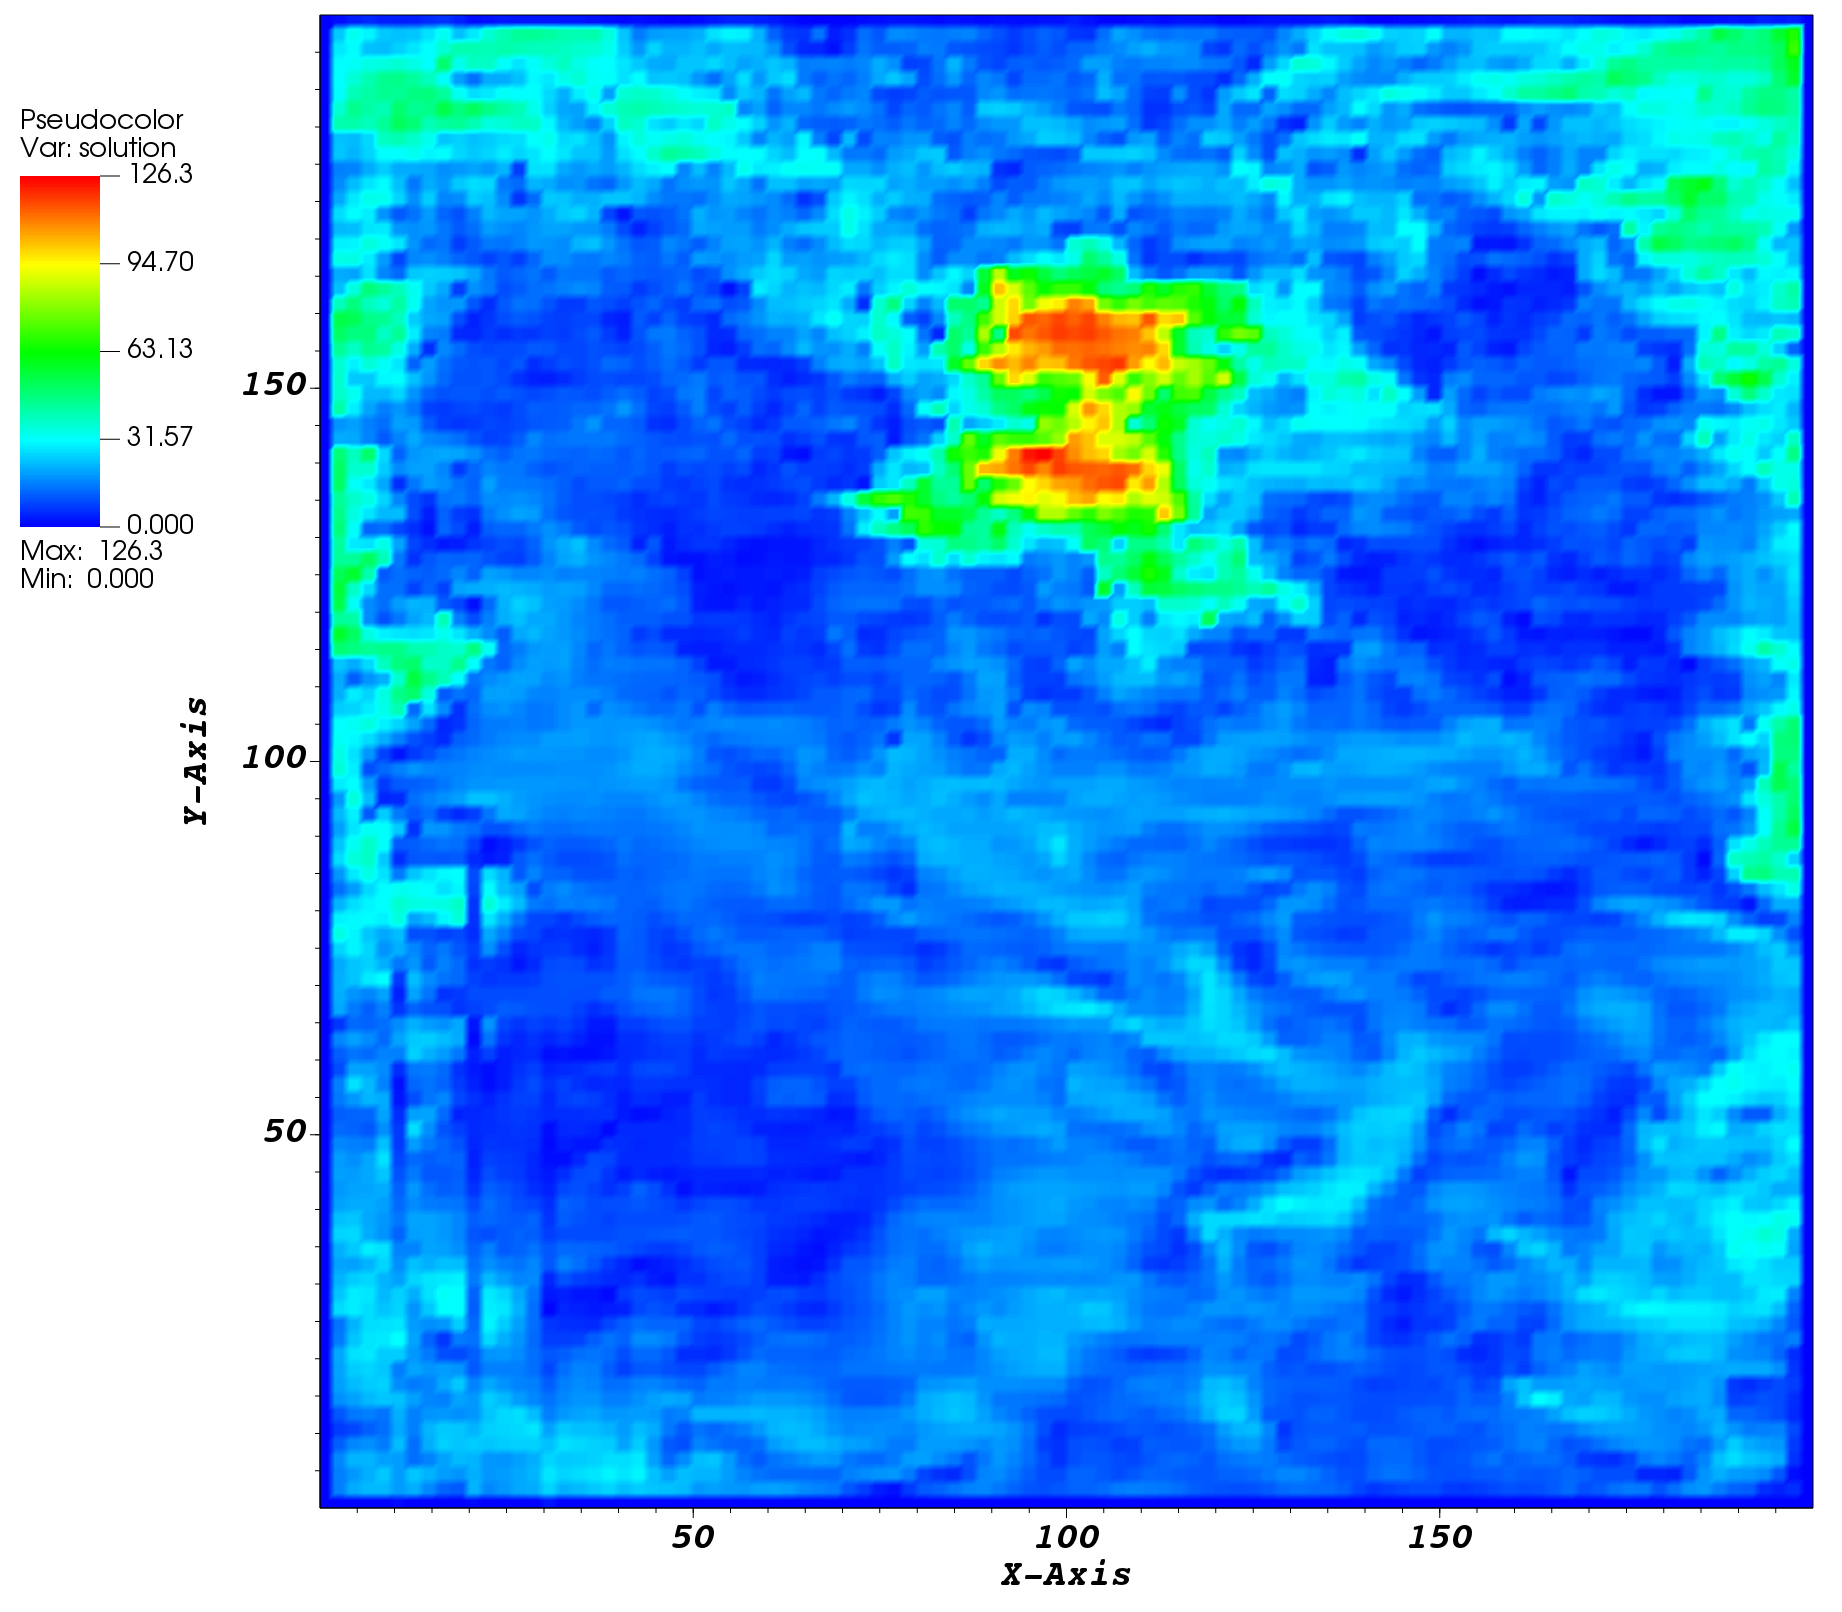
\includegraphics[width=0.33\textwidth]{figures/2d-nek-d6-n5-c20-aug6-reference.png}}
	\subfloat[Solution: 4x compression \label{fig:nek2d-d6-n5}]{%
		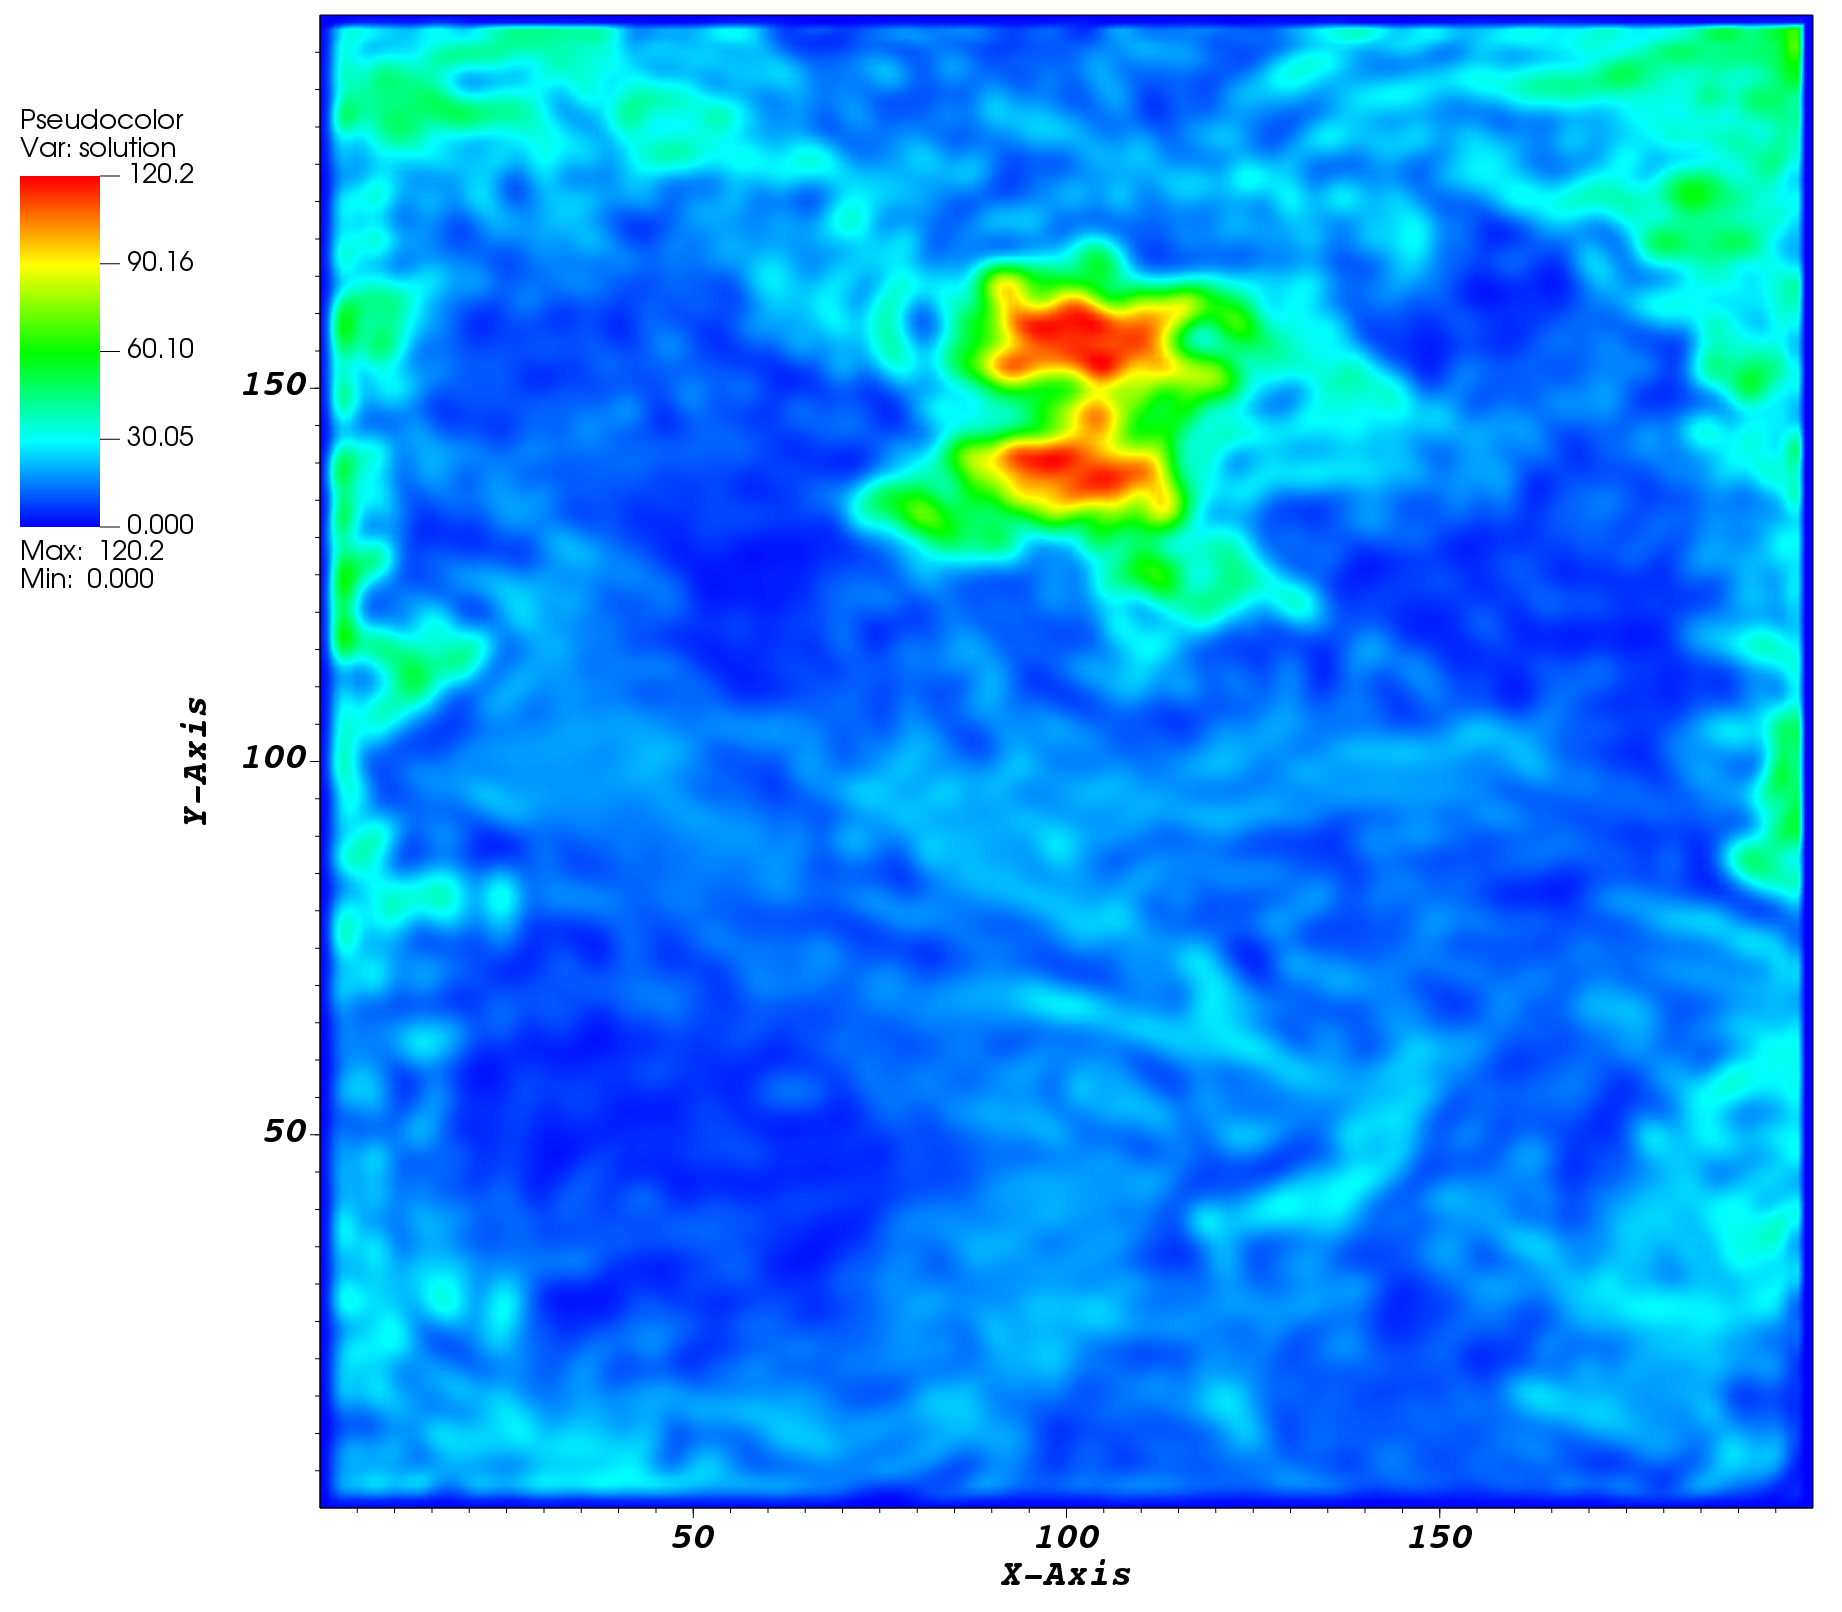
\includegraphics[width=0.33\textwidth]{figures/2d-nek-d6-n5-c20-aug6}}
	\subfloat[Solution: 1x compression\label{fig:nek2d-d6-n1}]{%
		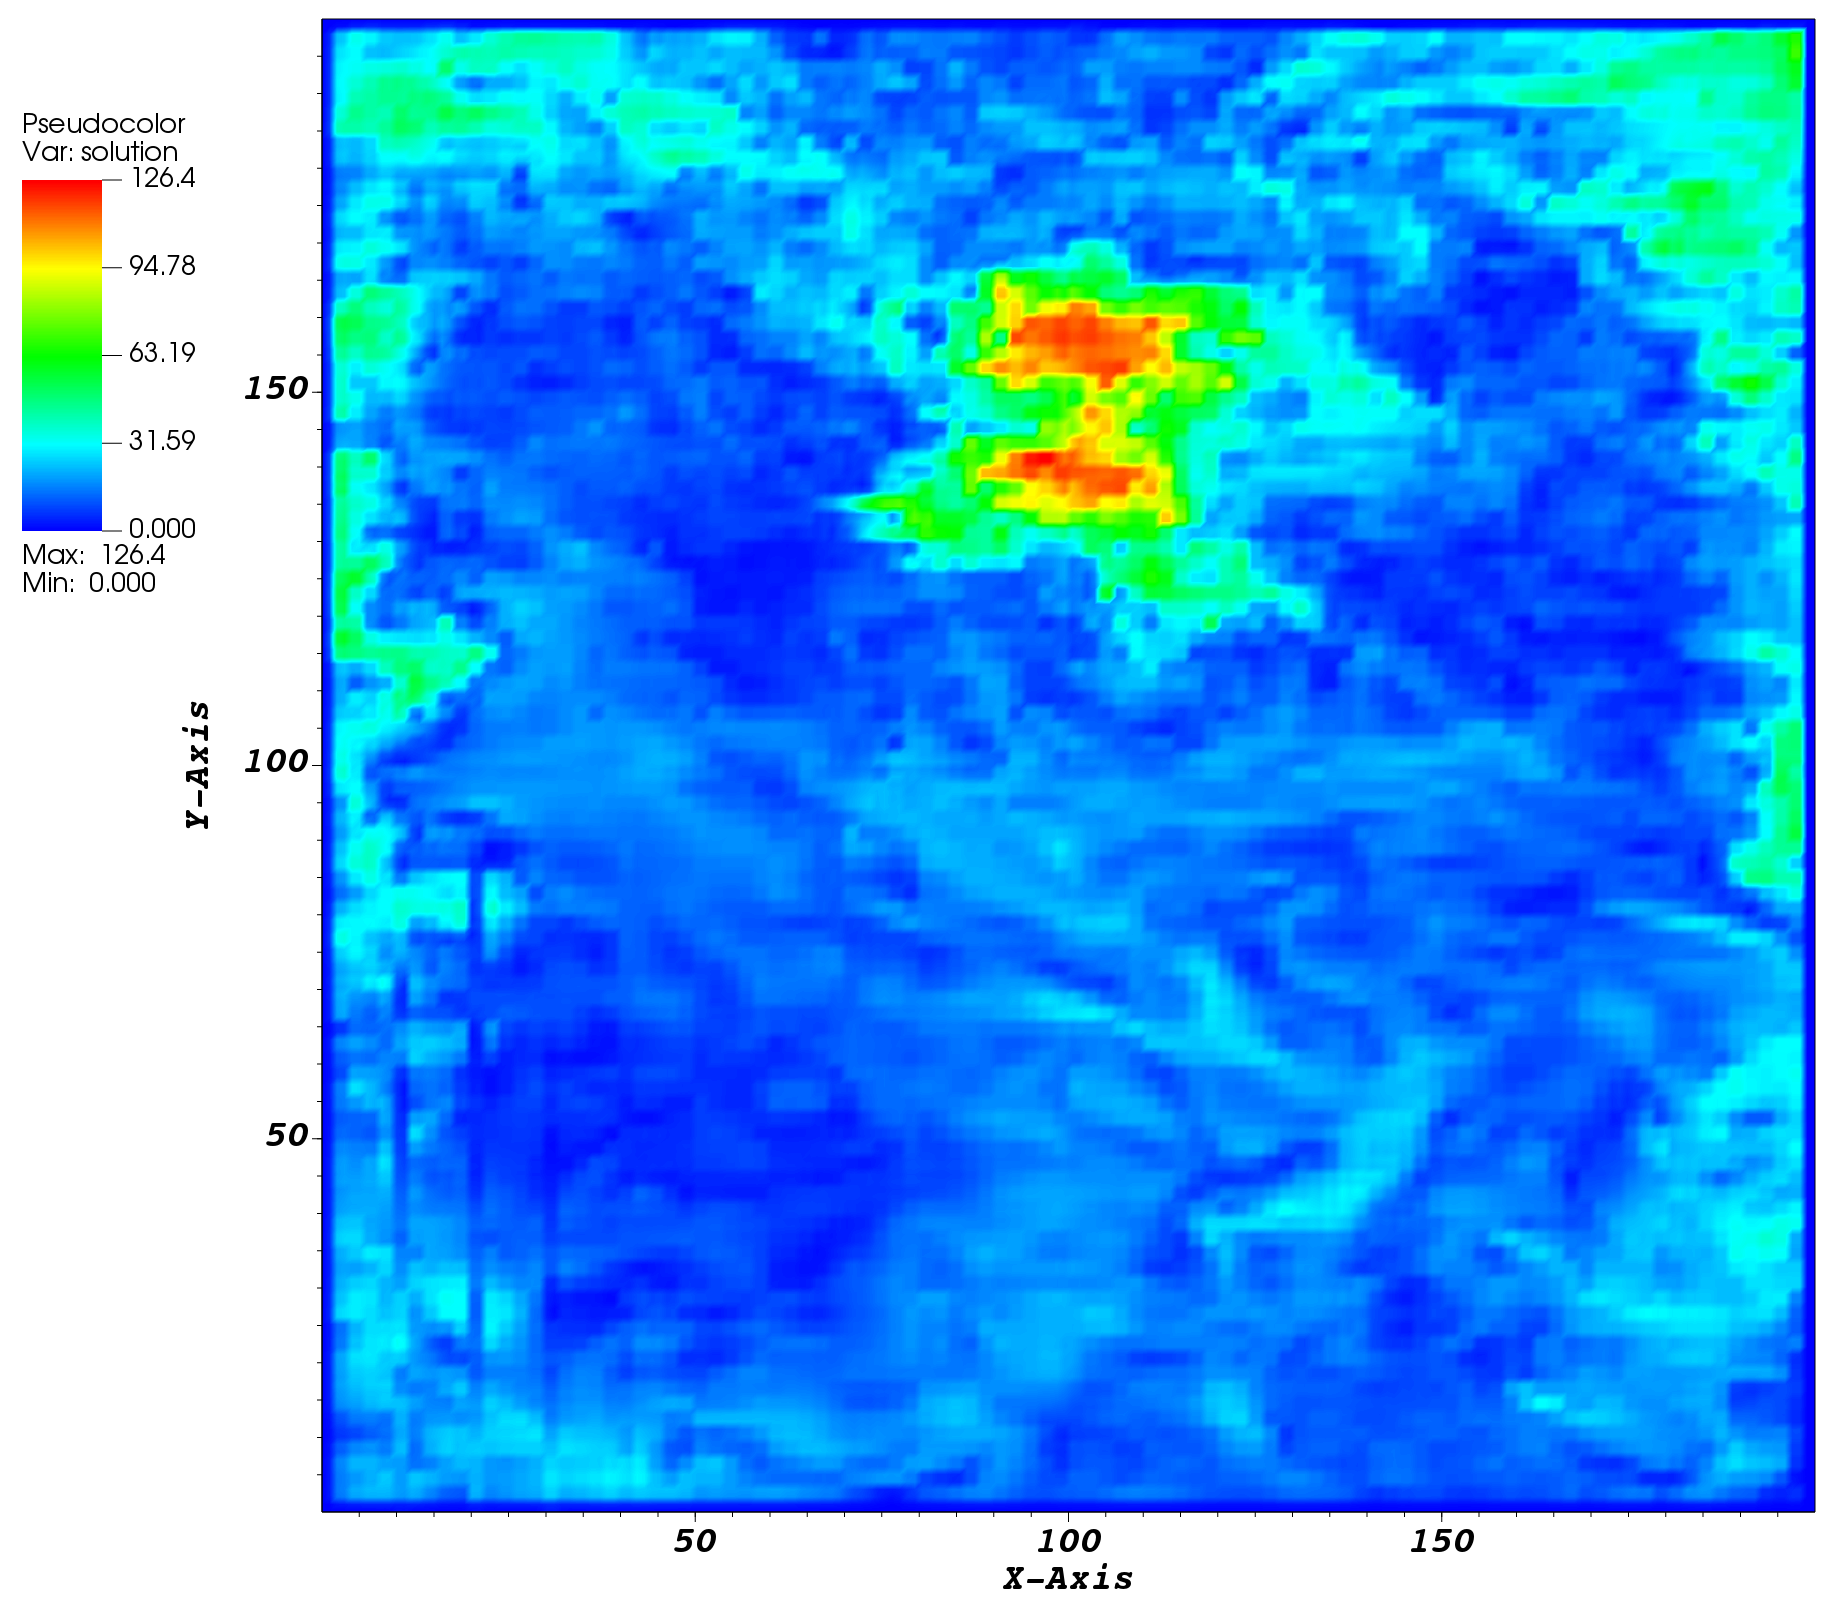
\includegraphics[width=0.33\textwidth]{figures/2d-nek-d6-n1-c200}}
	\caption{2D slice of the Nek5000 \dimension{3} dataset ($200 \times 200$): reference profile and B-spline MFA with $p=6$, $\mathcal{N}=5\times5$, $\left| \delta \right|=p$ for 4X compression (middle), and 1X compression (right).}
	\label{fig:nek2d-ref-reconstruct}
\end{figure}


\subsubsection{\dimension{3} Problem}

Next, we present S3D, a turbulent fuel jet combustion dataset generated from a simulation in the presence of an external cross-flow \cite{chen2009}. The \dimension{3} domain has the span $\left| \Omega \right|=704 \times 540 \times 550$, with the raw data containing three components of the vector field. We choose to use the magnitude of this velocity field in our reconstruction study shown below in \fig{fig:s3d-ref-error} with 209M points. The converged MFA reconstruction shown in the figure with $8^3=512$ subdomains and $n=35$ per direction  in each subdomain yields a net compression ratio of $\frac{(704\times540\times550)}{(8\times35)^3} \approx 9.5$. While uniform refinement in knot spans does yield sufficient error reductions in most subdomains, utilizing adaptive error resolution with knot insertions and removals for MFA as previously used here for single subdomains \cite{nashed-rational} for the S3D problem can provide better reconstructions in addition to the iterative scheme introduced here. Such extensions will be pursued in the future. However, the experiments demonstrate that the MFA computations produce reconstructed data and  numerical errors that are consistent and convergent for arbitrary $\mathcal{N}, n, p$ and values of $\left| \delta \right|$, proving the feasibility of the algorithm.

\begin{figure}[htbp]
	\centering
	\subfloat[S3D dataset profile\label{fig:s3d-refprofile}]{%
		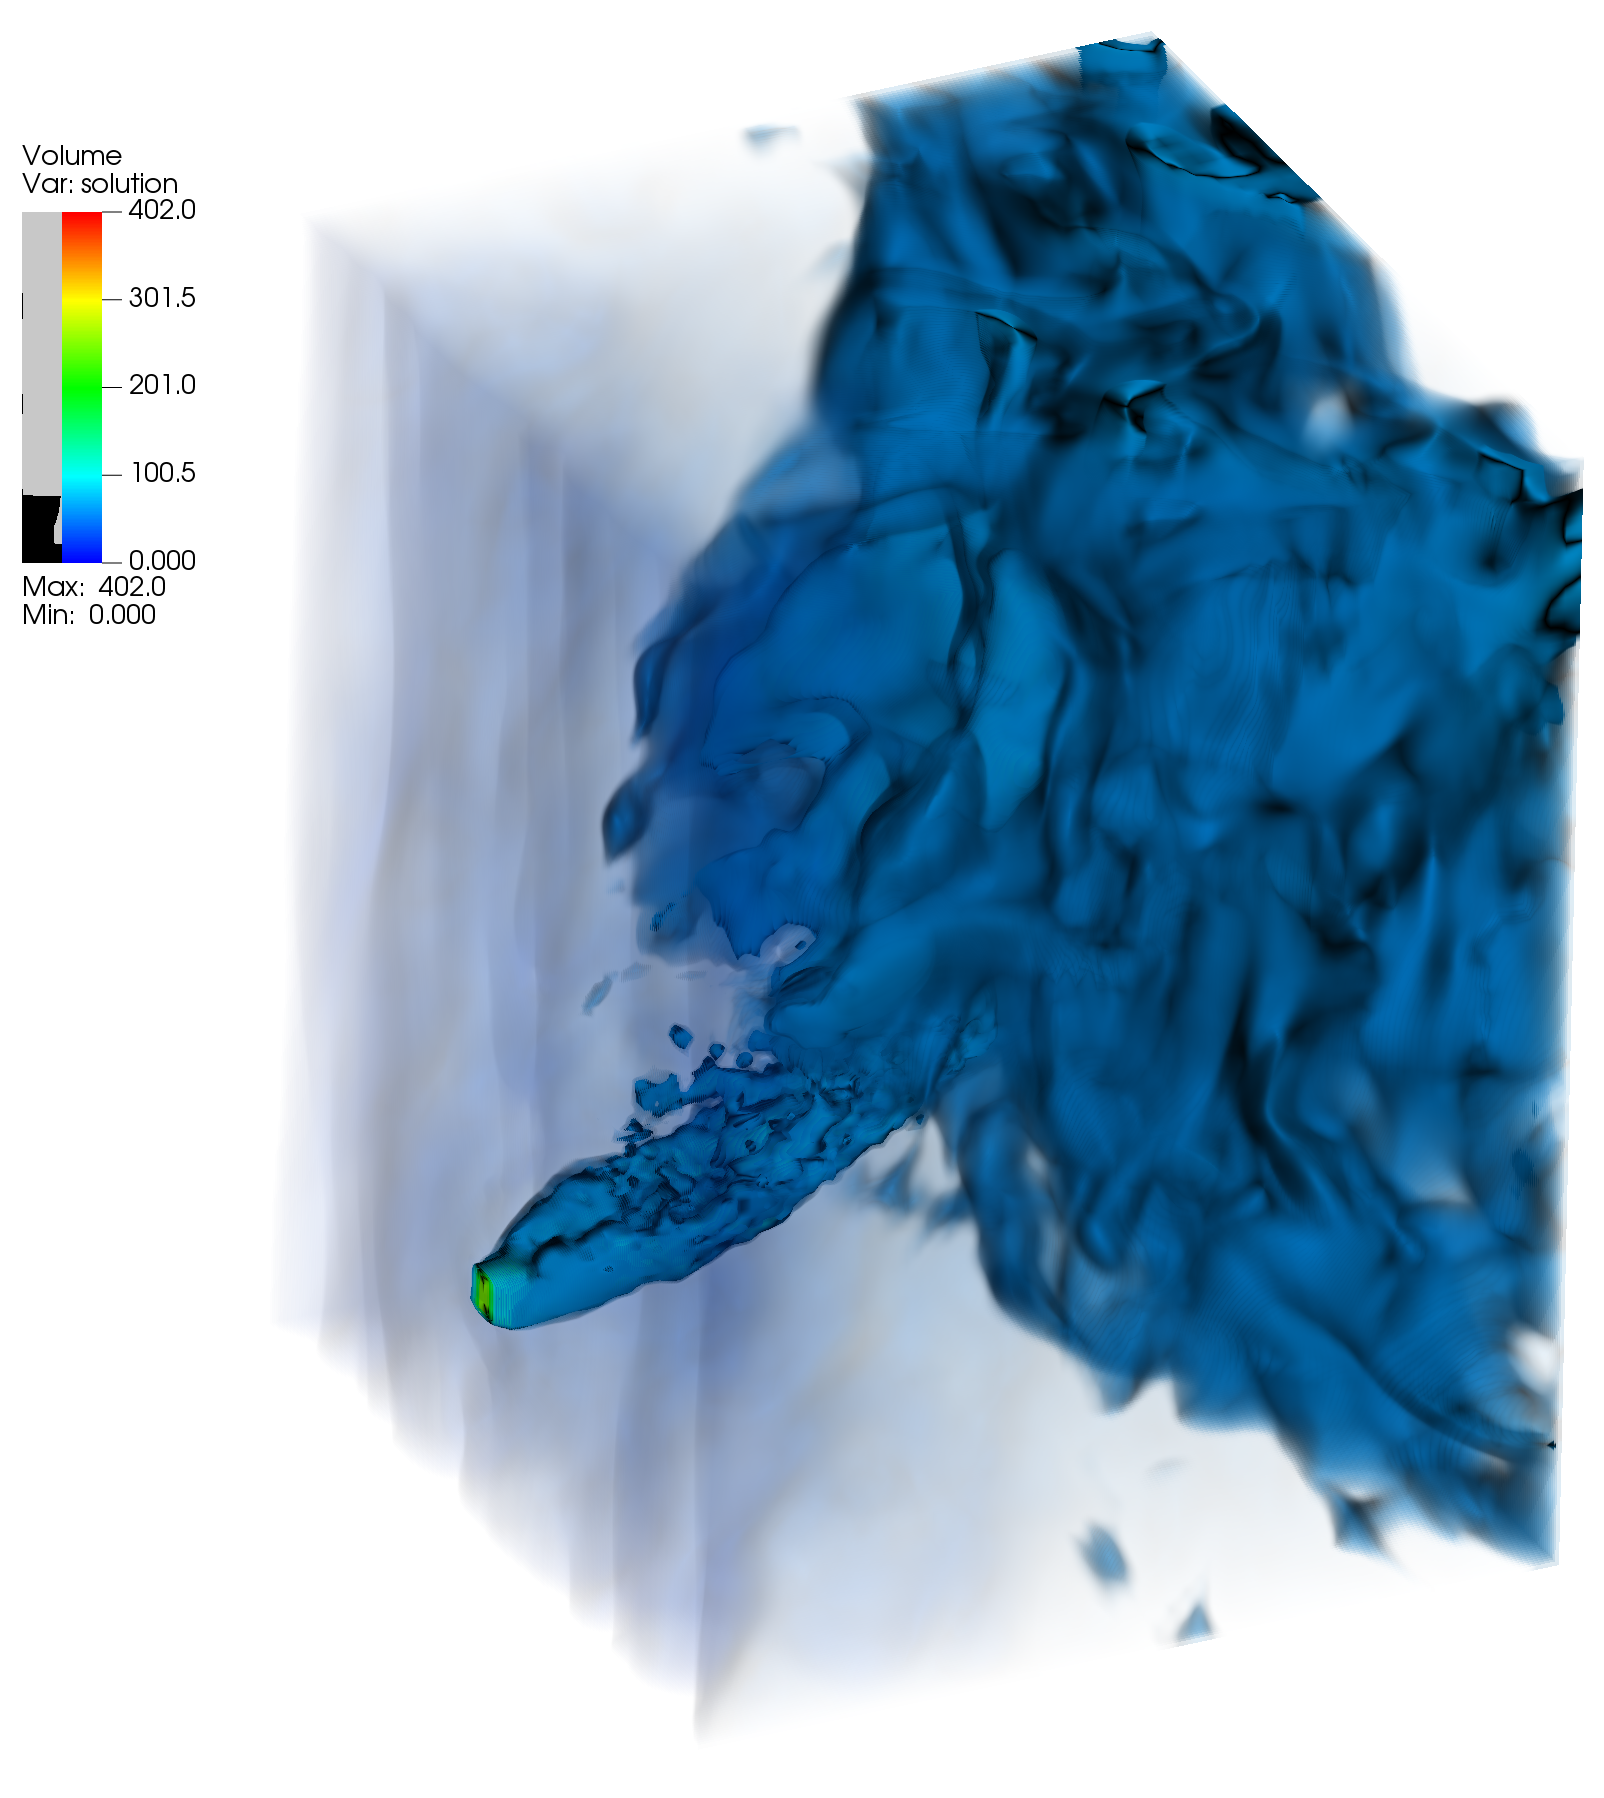
\includegraphics[width=0.33\textwidth]{figures/s3d-volume-profile-reference3.png}}
	\subfloat[Converged solution profile\label{fig:s3d-profile}]{%
			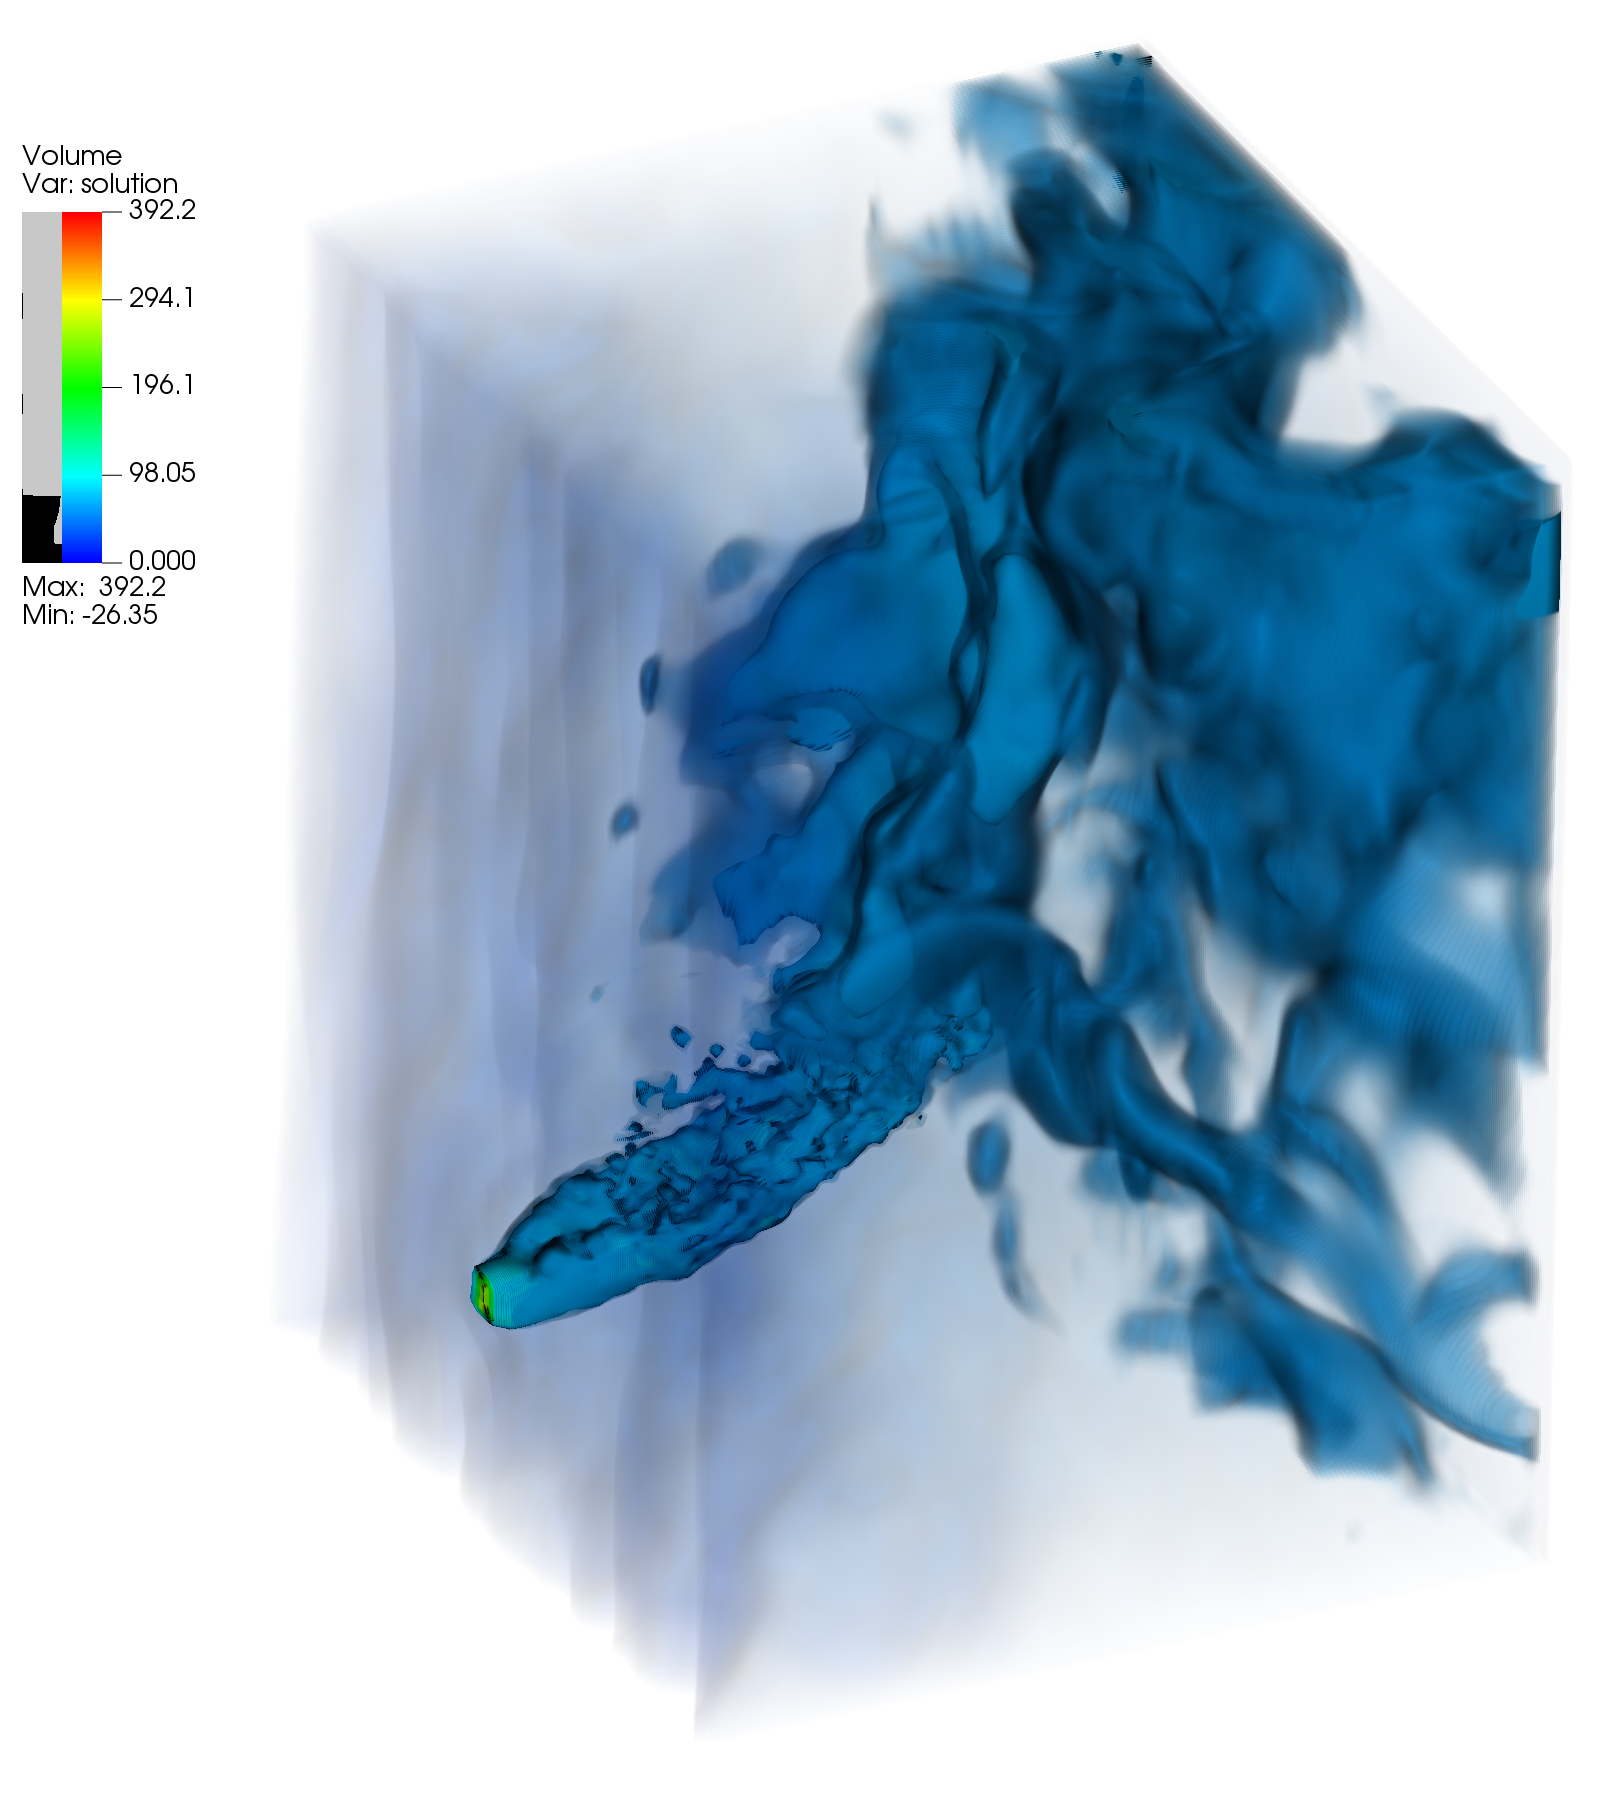
\includegraphics[width=0.33\textwidth]{figures/s3d-volume-profile-conv3.png}}
	\subfloat[Final error profile\label{fig:s3d-error}]{%
	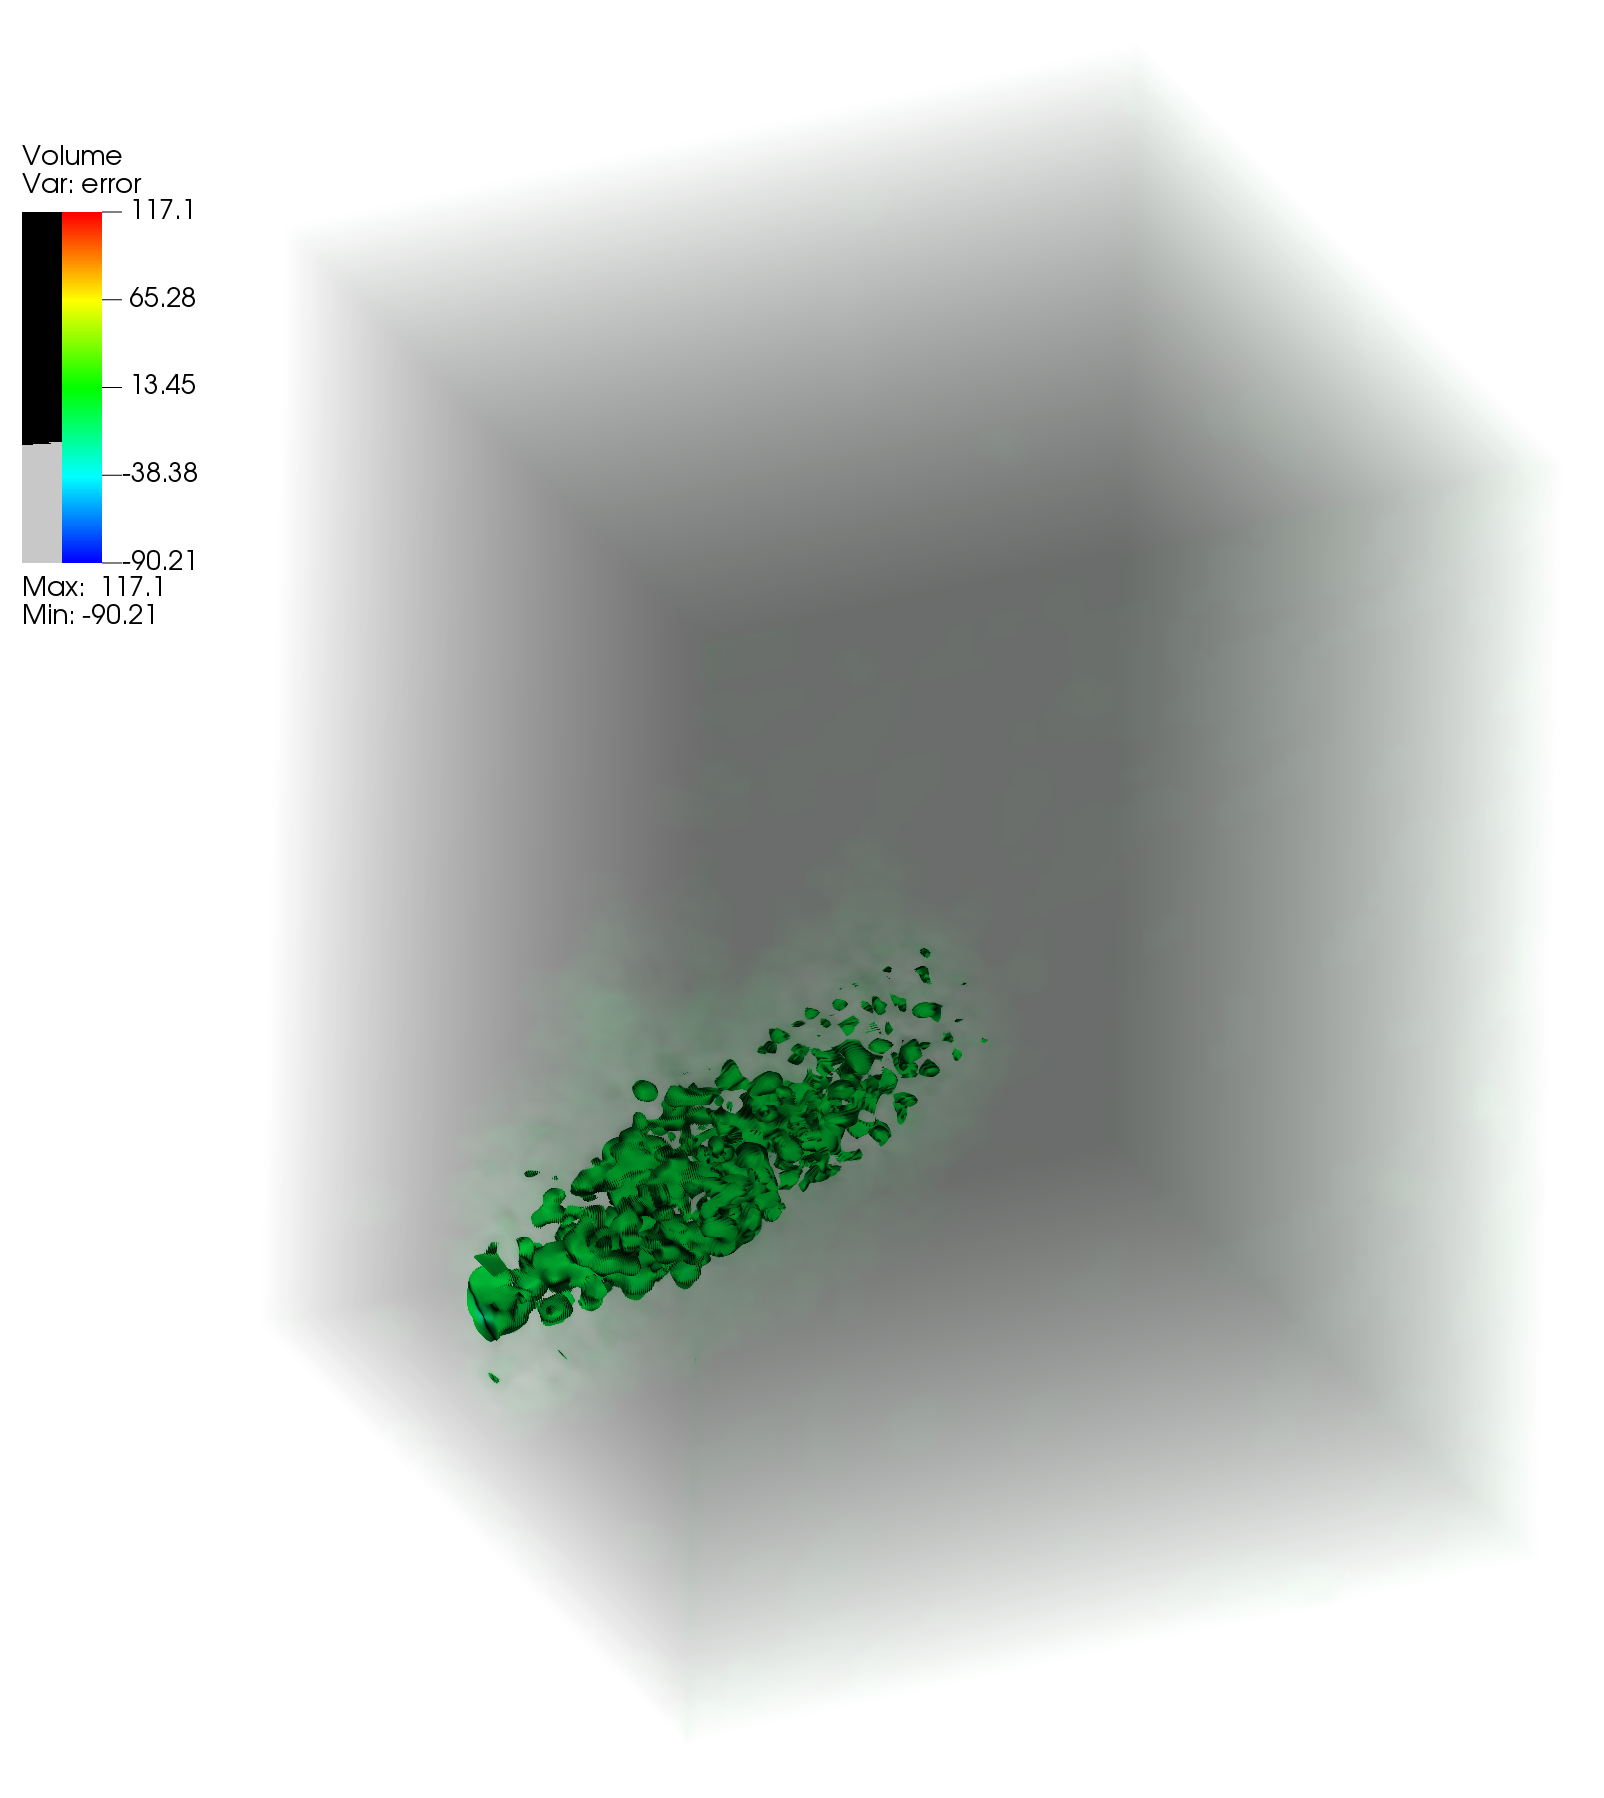
\includegraphics[width=0.33\textwidth]{figures/s3d-volume-profile-error-conv3.png}}
	\caption{Volume rendered S3D dataset with 9.5X compression: reference profile, converged MFA decoded profile and the corresponding reconstruction error with $\mathcal{N}=8\times 8\times 8=512$, $p=3$ and  $\left| \delta \right|=2p=6$}
	\label{fig:s3d-ref-error}
\end{figure}


\subsubsection{Error Convergence}

%\comment{Show error convergence in \dimension{3} problem to look at how iteratively things resolve}

We utilize synthetic datasets shown in \eqt{eqt:2d-synthetic} and \eqt{eqt:3d-synthetic} to perform error convergence studies and to determine areas of maximal error that iteratively are resolved between neighboring subdomains.

%\vspace*{-4mm}
%
%\begin{equation}
%	F(x,y)  = sinc(\sqrt{x^2+y^2}) + sinc(2(x - 2)^2 + 2(y + 2)^2), \forall (x,y) \in [-4,4]^2
%	\label{eqt:2d-synthetic}
%\end{equation}
%
%\vspace*{-8mm}
%
%\begin{equation}
%	F(x,y,z) = sinc(\sqrt{x^2 + y^2 + z^2}) + sinc(2(x - 2)^2 + (y + 2)^2 + (z - 2)^2), \forall  (x,y,z) \in [-4,4]^d.
%	%\\
%	%\quad \quad &\forall& \Omega = (x,y,z) \in [-4,4]^d.
%	\label{eqt:3d-synthetic}
%\end{equation}


\begin{eqnarray}
	F(x,y)  &=& sinc(\sqrt{x^2+y^2}) + sinc(2(x - 2)^2 + 2(y + 2)^2), \forall (x,y) \in [-4,4]^2, \label{eqt:2d-synthetic}\\
	\quad \quad F(x,y,z) &=& sinc(\sqrt{x^2 + y^2 + z^2}) + sinc(2(x - 2)^2 + (y + 2)^2 + (z - 2)^2), \forall  (x,y,z) \in [-4,4]^d.
	\label{eqt:3d-synthetic}
\end{eqnarray}

We plot the change in error $\vec{E}$ between subsequent iterations of the RAS scheme for both \dimension{2} and \dimension{3} problem cases with $\left| \delta \right|=0$ in \fig{fig:2d-3d-error-convergence}. This clearly demonstrates that the $\mathcal{SS}$ interface values are resolved first, and then $\mathcal{MS}$ DoFs are resolved further. In all cases, the iterations converge in 2 steps, independent of $\mathcal{N}$ or $\delta$.
%
\begin{figure}[htbp]
	\centering
	\subfloat[\dimension{2} problem with $\mathcal{N}=5\times 5$: Iteration 1\label{fig:2d-iter1}]{%
		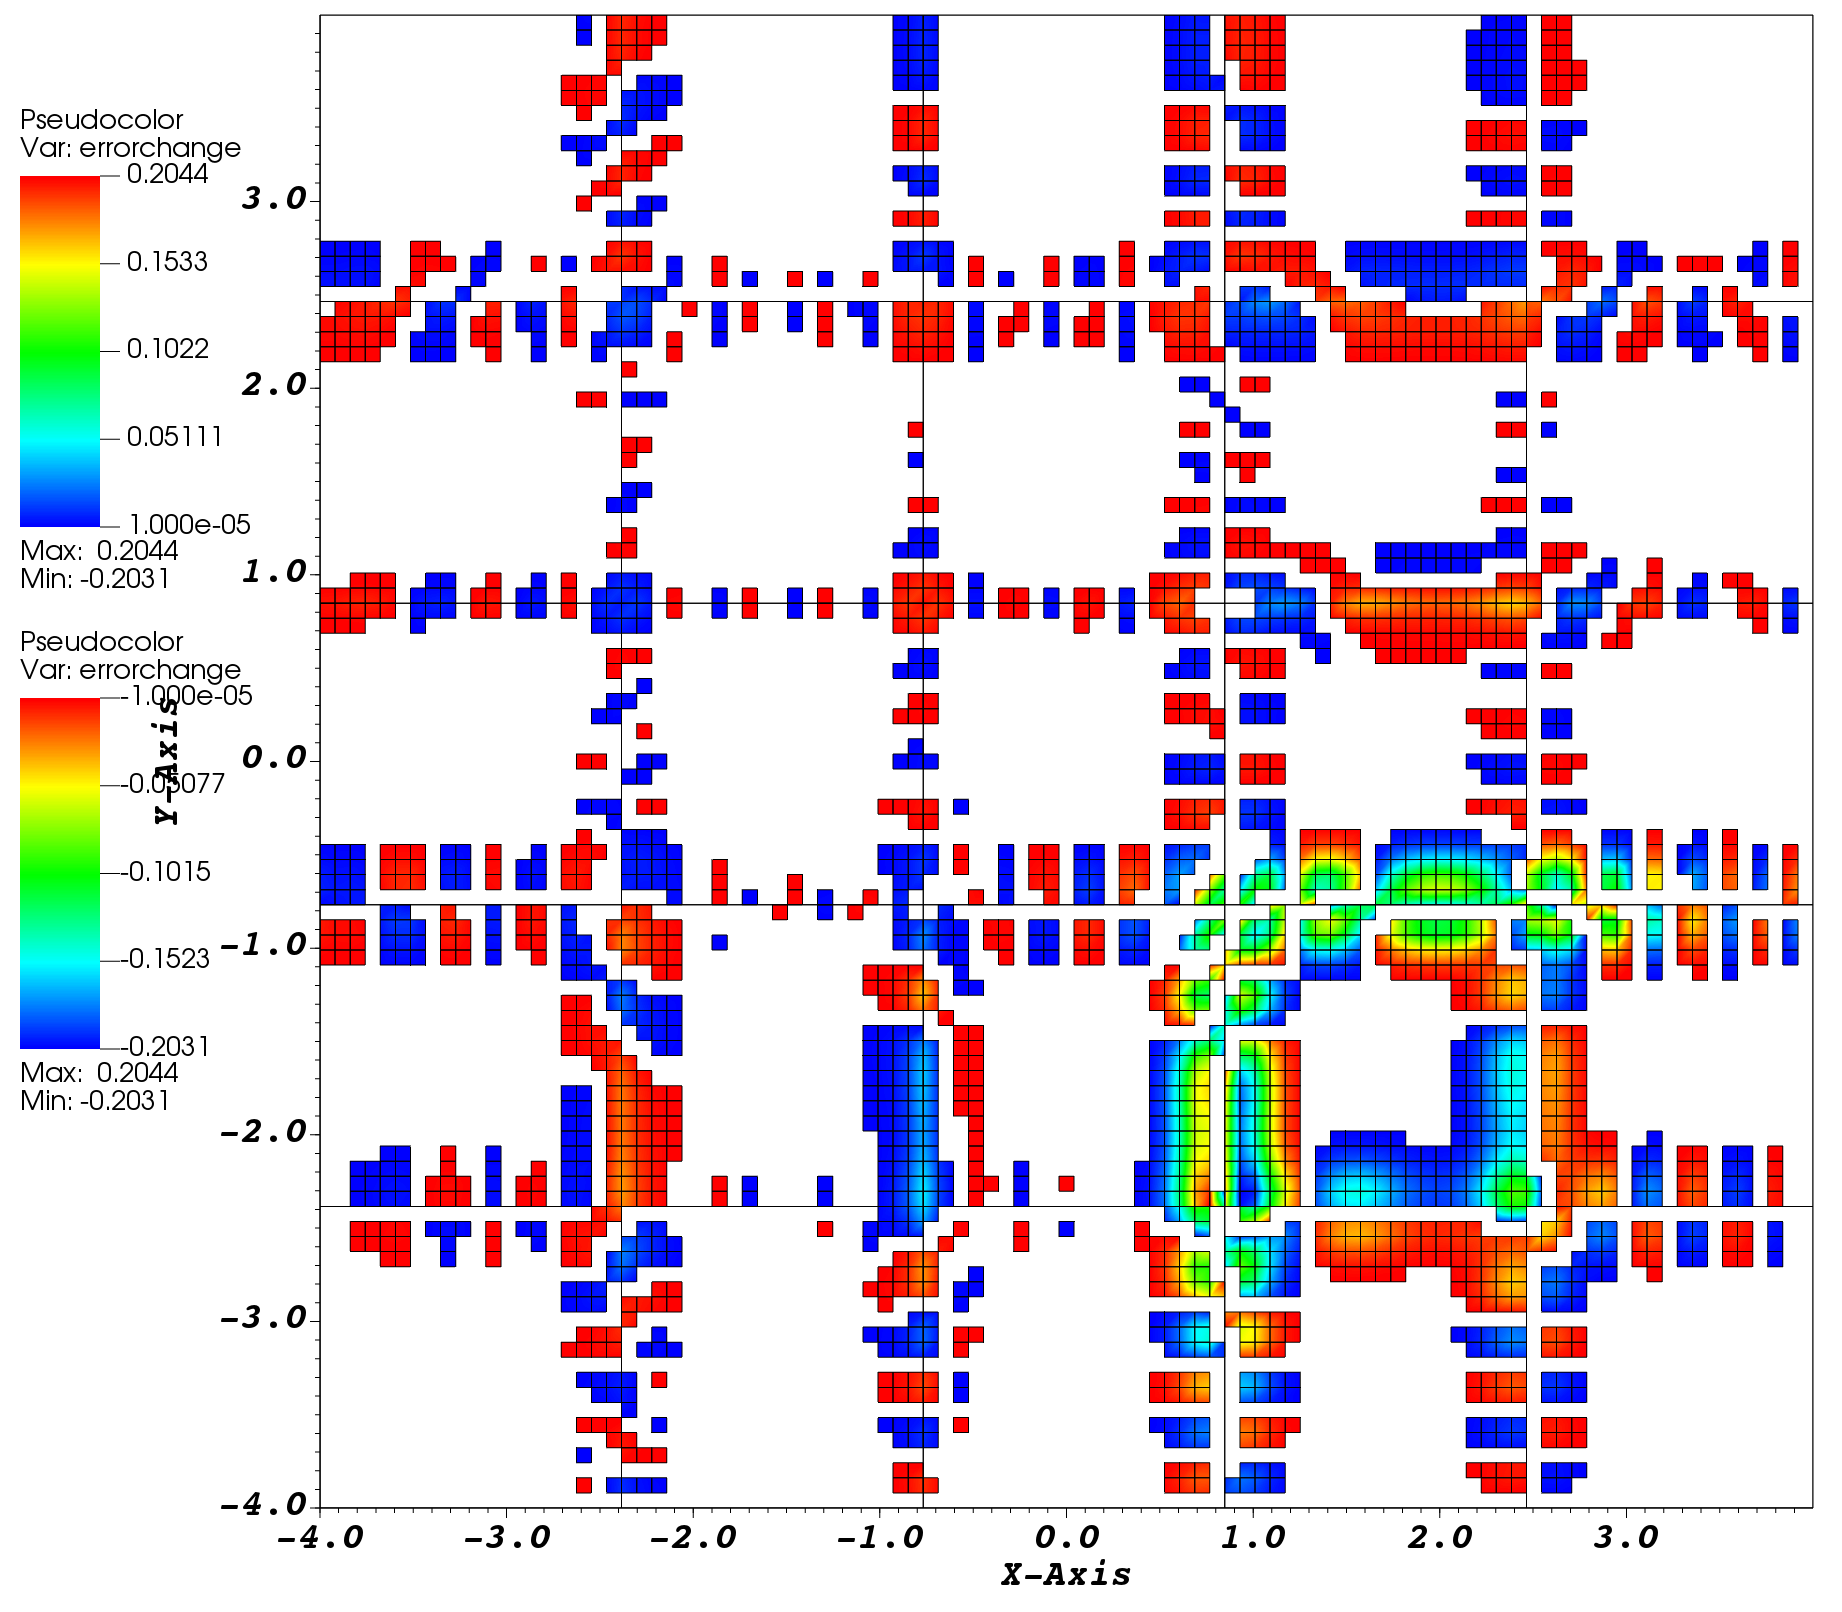
\includegraphics[width=0.44\textwidth]{figures/2d-d3-n5-aug0-iter1-threshold0001.png}}
	\quad \quad
	\subfloat[\dimension{2} problem with $\mathcal{N}=5\times 5$: Iteration 2\label{fig:2d-iter2}]{%
		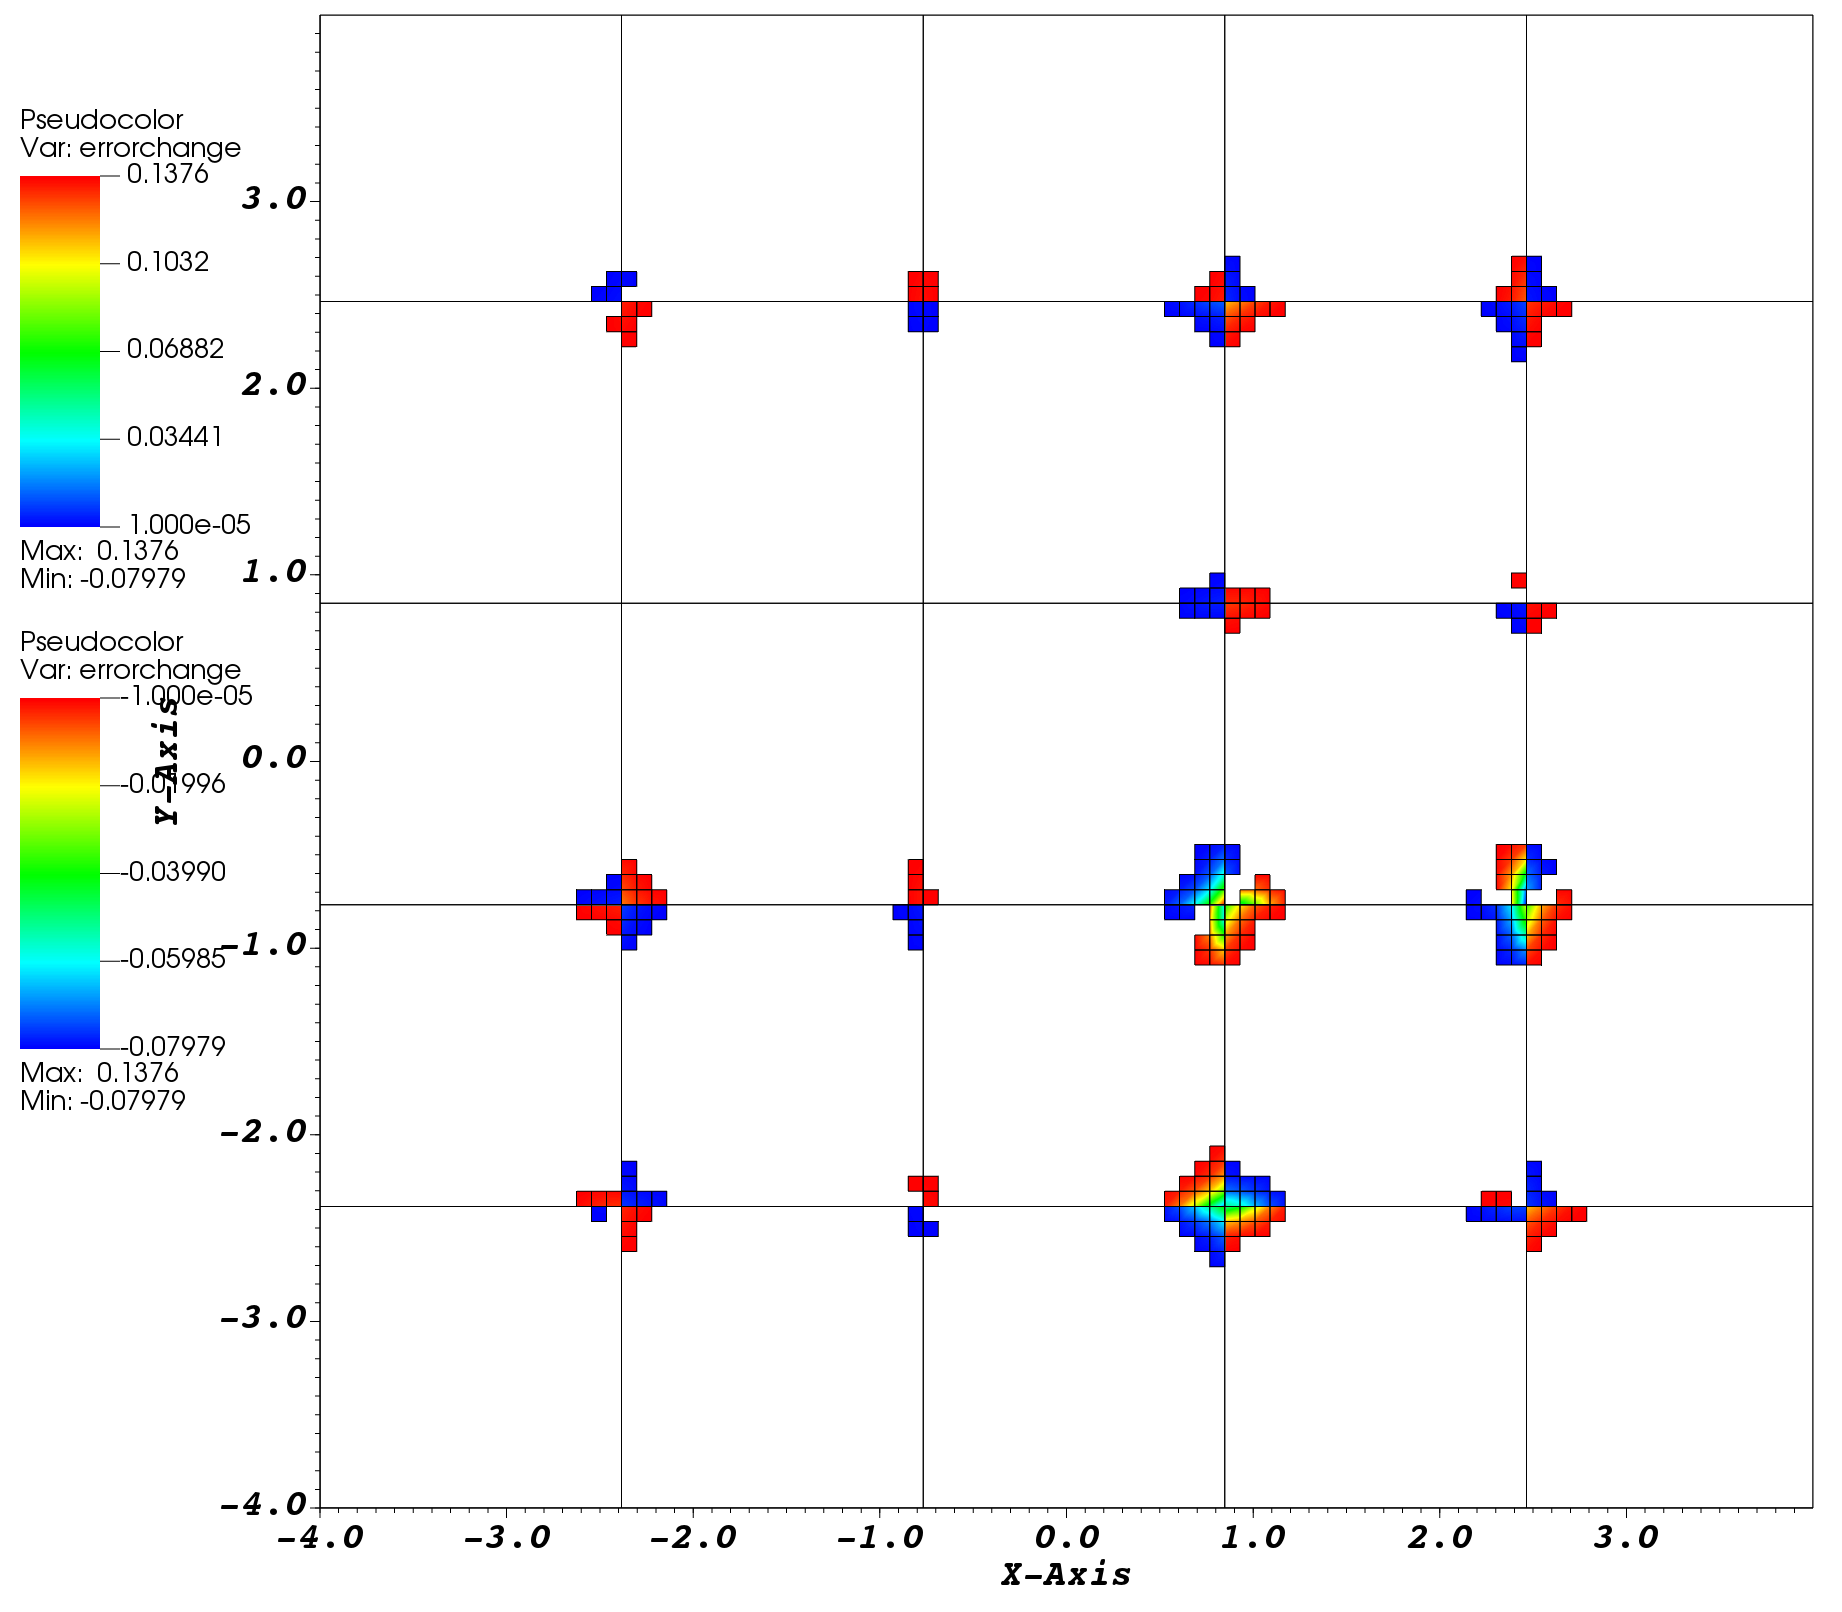
\includegraphics[width=0.44\textwidth]{figures/2d-d3-n5-aug0-iter2-threshold0001.png}}\\
	\subfloat[\dimension{3} problem with $\mathcal{N}=3\times 3 \times 3$: Iteration 1\label{fig:3d-iter1}]{%
	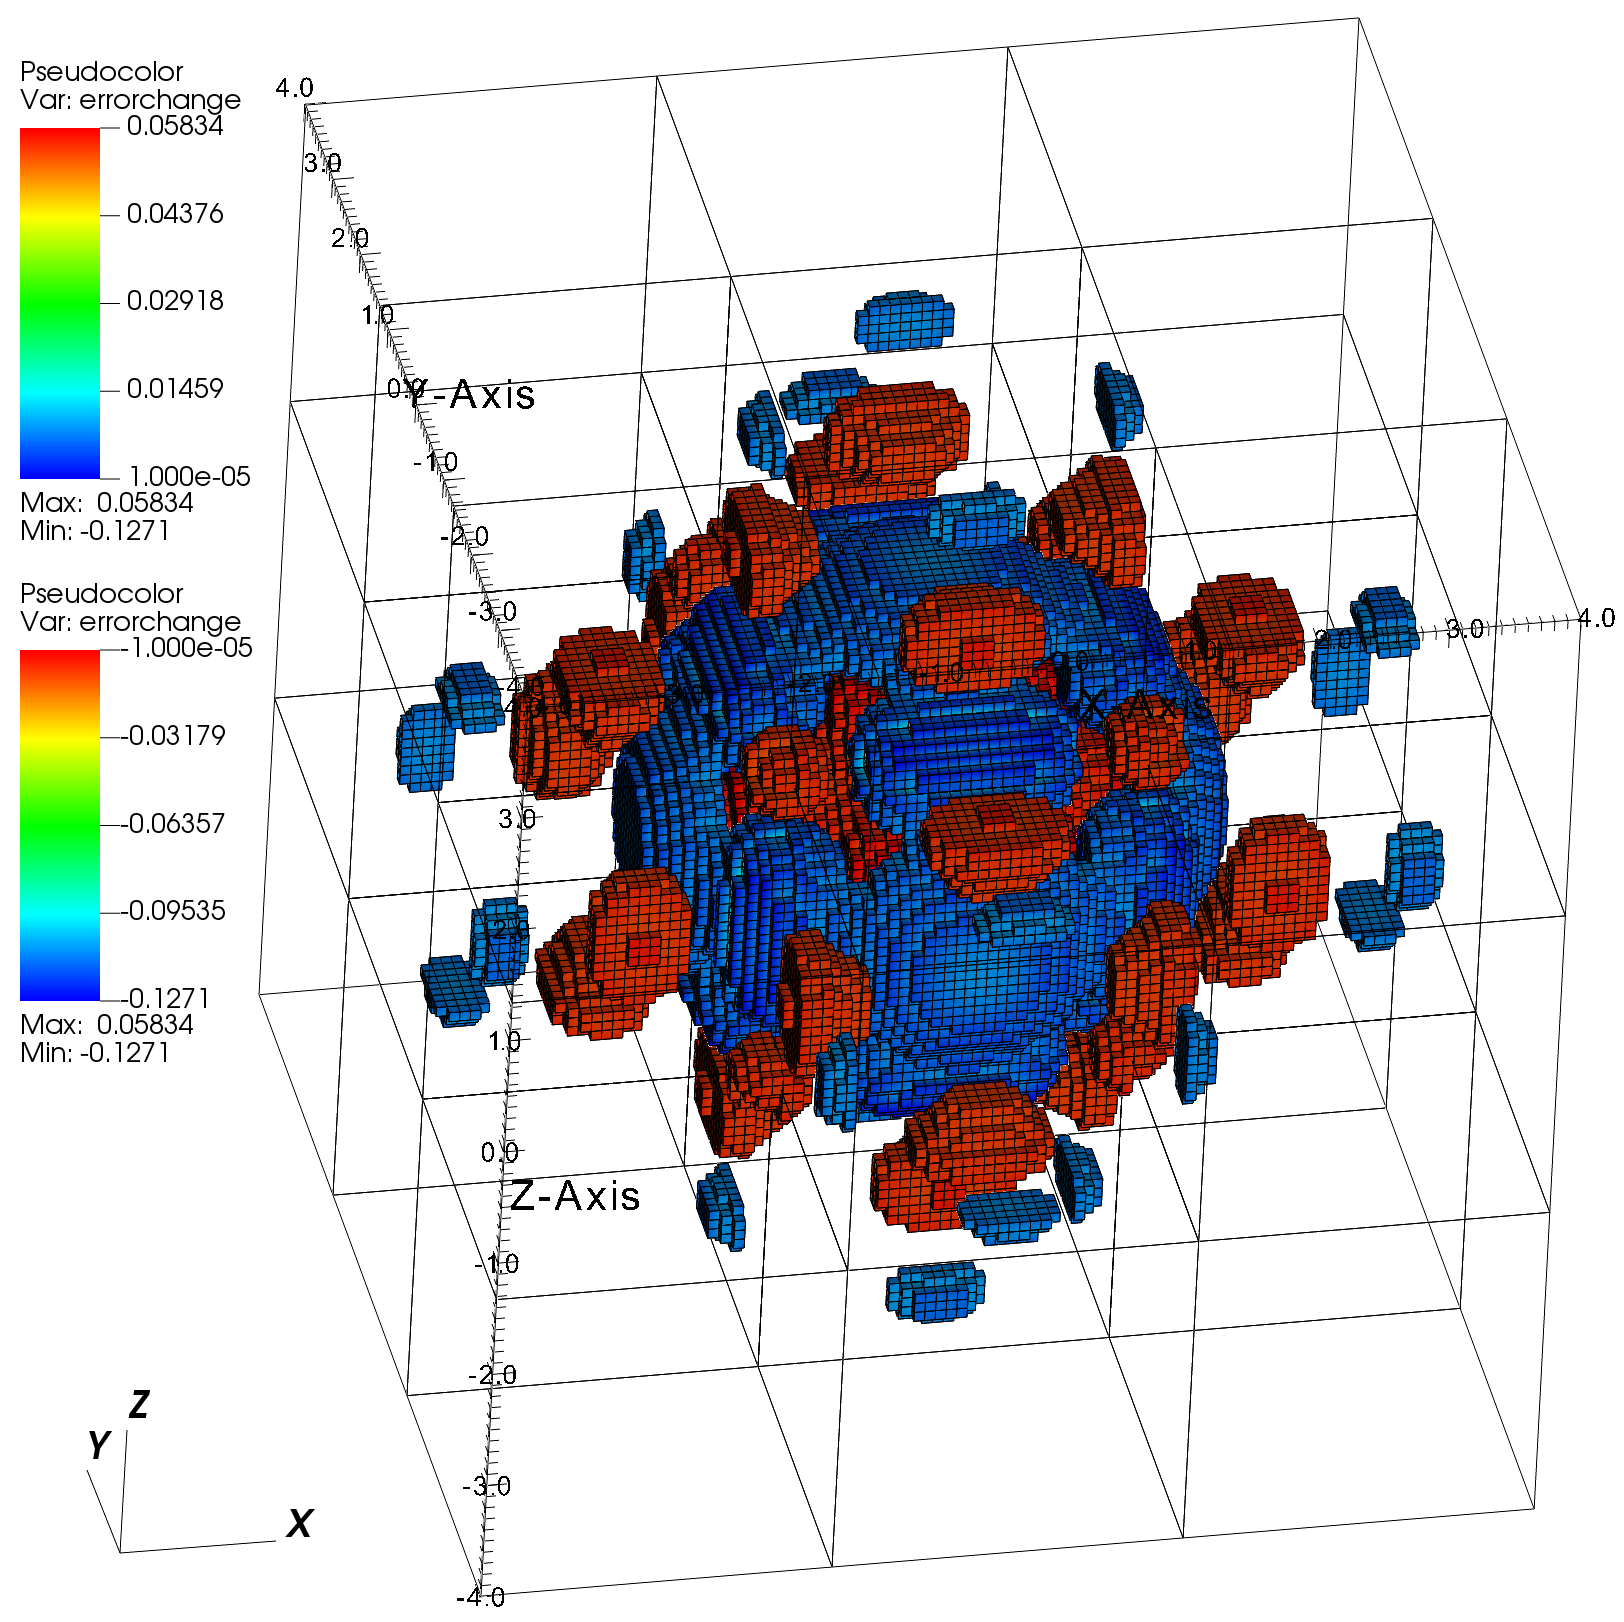
\includegraphics[width=0.44\textwidth]{figures/3d-d5-n4-aug0-iter1-threshold01.png}}
	\quad \quad
	\subfloat[\dimension{3} problem with $\mathcal{N}=3\times 3 \times 3$: Iteration 2\label{fig:3d-iter2}]{%
	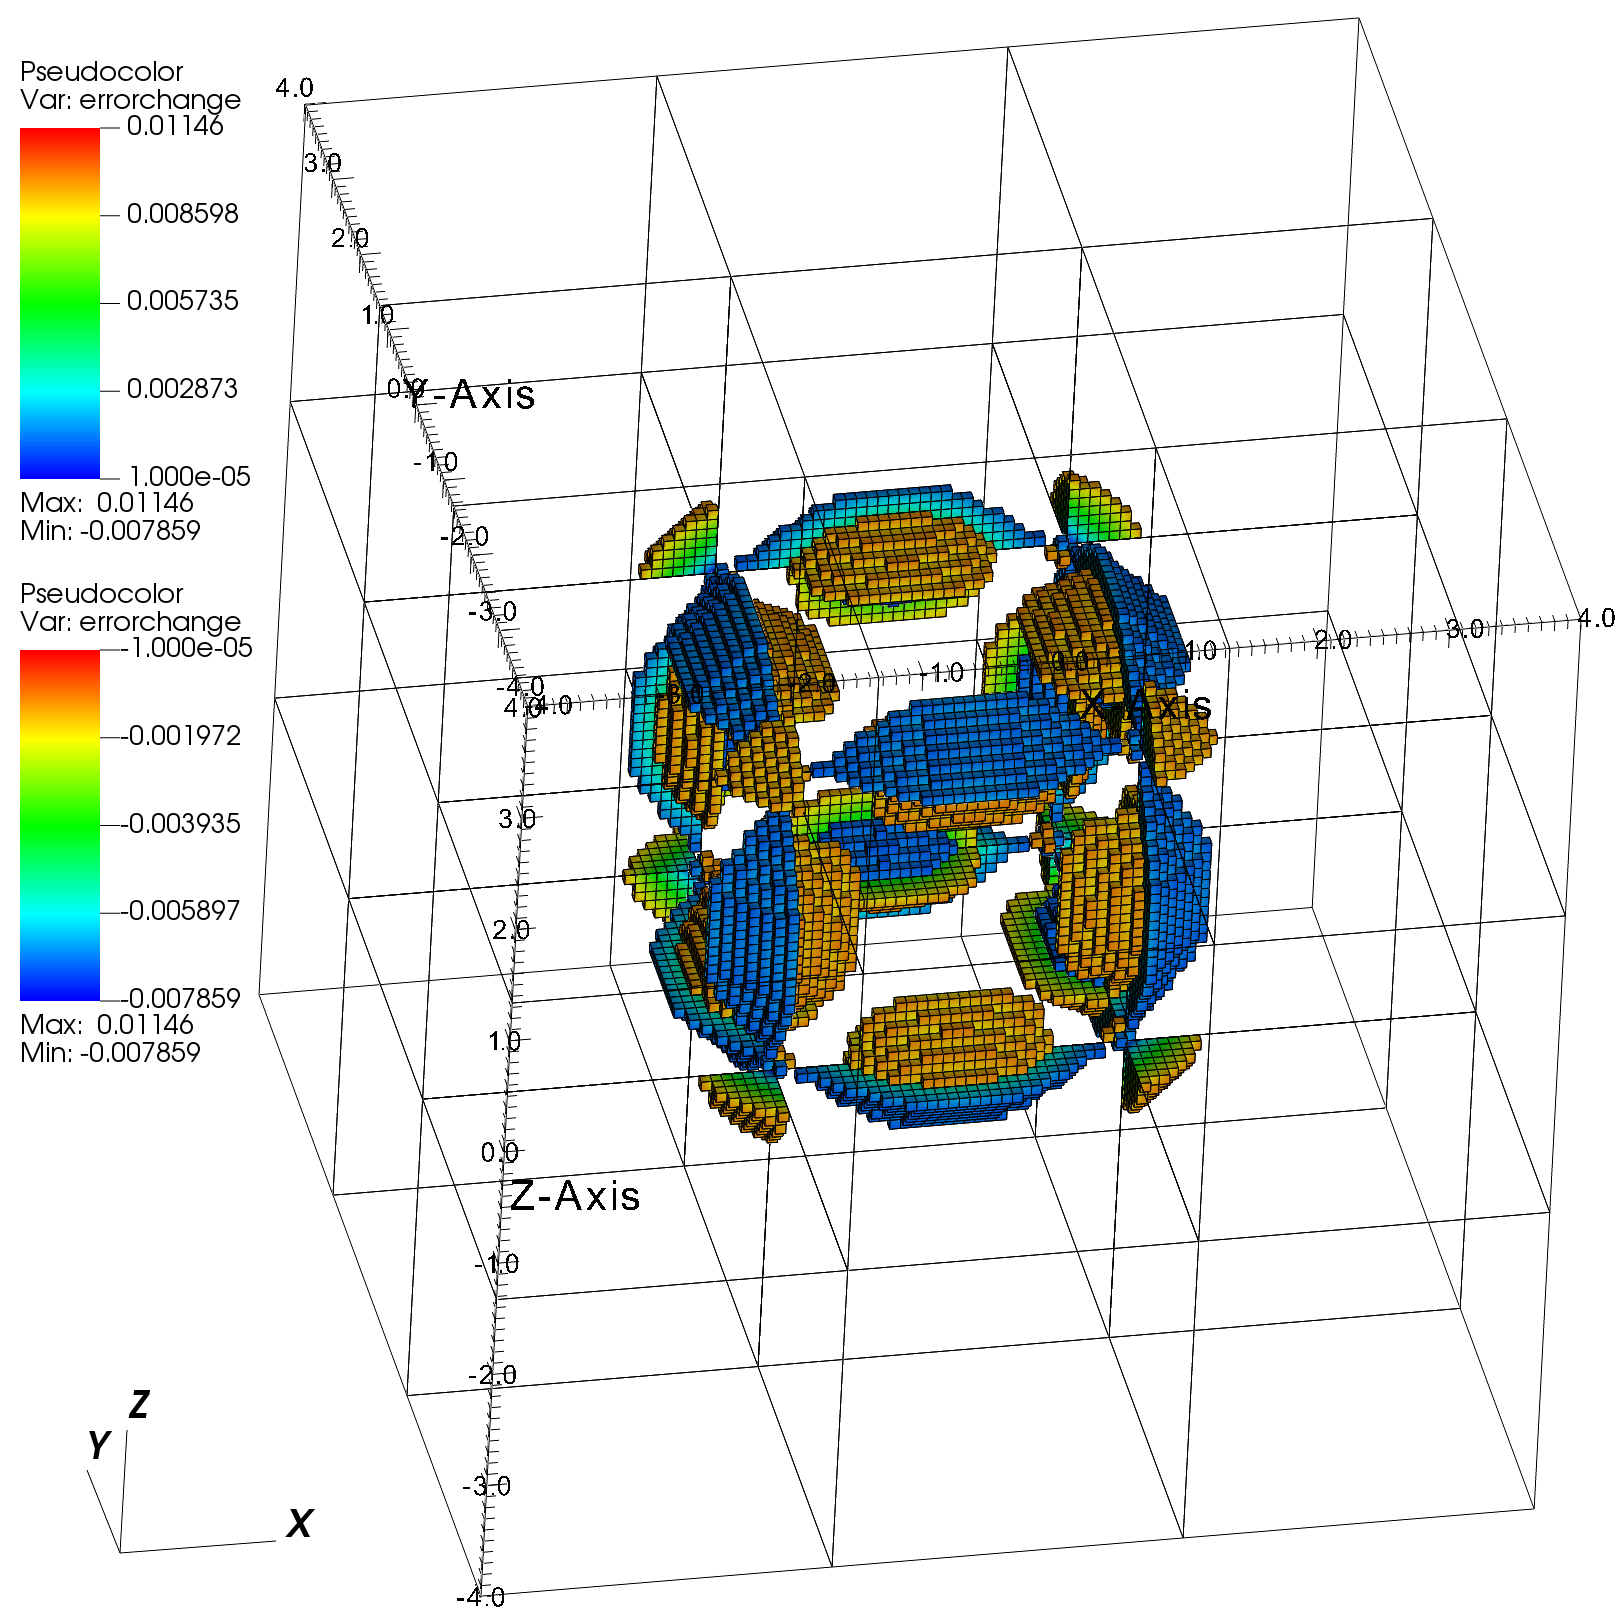
\includegraphics[width=0.44\textwidth]{figures/3d-d5-n4-aug0-iter2-threshold001.png}}\\
	\caption{Error convergence for \dimension{2} and \dimension{3} problems on the first and second iterate}
	\label{fig:2d-3d-error-convergence}
\end{figure}



%Using the 2-D sinc analytical function, the error convergence for different NURBS bases degree $p$ was measured. As the number of control point DoFs are increased, the global norm of the errors are reduced consistently in the current implementation. Next we tested the spatial adaptivity in 2-D on a scientific dataset to ensure that the hierarchical iterative scheme with RAS is able to capture strong solution variations, and still ensure continuity across subdomain interfaces. 
%Using varying fidelity of the real world data, and the ability to create complex closed form functionals within our Python implementation, the approach was verification for accuracy using uniform control point refinements to yield sizes theoretical convergence orders. 
%We utilize the described 2-D problem datasets to better understand the convergence and parallel scalability of the proposed algorithms at scale. Demonstrations for the S3D, and CESM datasets are provided below.

%\subsubsection{S3D Dataset: Spatial Adaptivity}

%Additionally, using adaptive resolution based on a-posteriori gradient estimates, numerical errors in strongly varying solution profiles were reduced to within user-specified tolerances. A sample solution for the 2-D slice of the S3D dataset on 9 subdomains is shown in \fig{fig:s3d-adaptive-2d}, along with the error profiles at the first iteration in \fig{fig:s3d-adaptive-2d-b} and on convergence of the RAS iterations in {fig:s3d-adaptive-2d-c}.
%
%\begin{figure}[htbp]
%	\centering
%	\subfloat[S3D dataset profile\label{fig:s3d-adaptive-2d-a}]{%
%	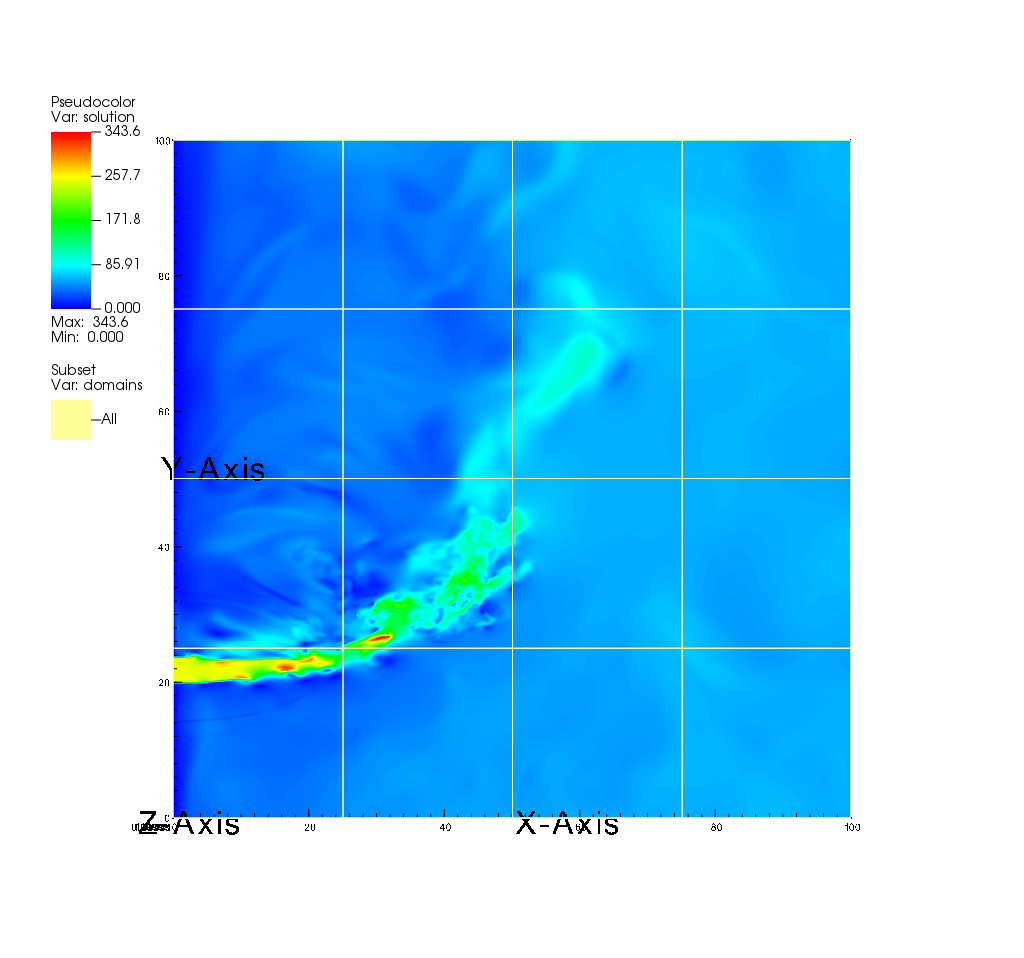
\includegraphics[width=0.44\textwidth]{figures/s3d-2d-profile.png}}
%	\hfill
%	\subfloat[Error profile before RAS iteration or adaptivity\label{fig:s3d-adaptive-2d-b}]{%
%		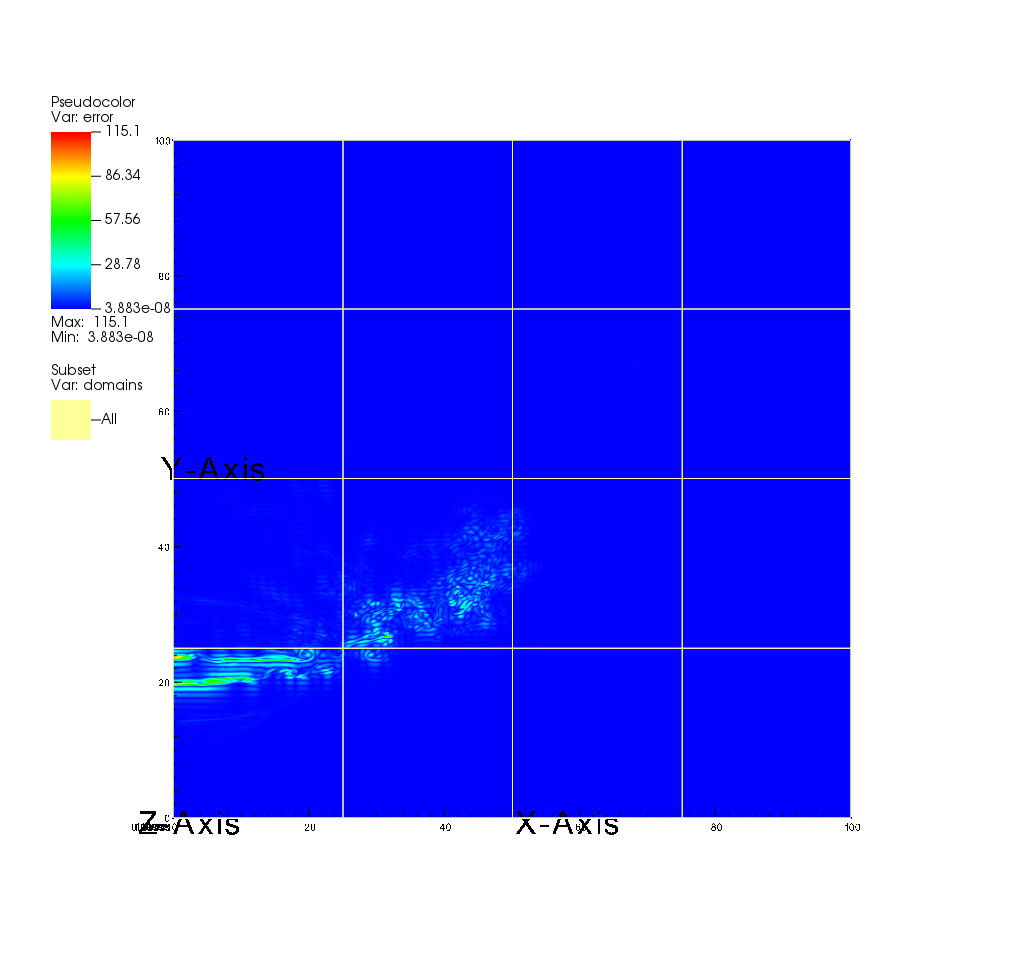
\includegraphics[width=0.44\textwidth]{figures/s3d-error-iter1}}\\
%	\subfloat[Error profile after RAS iteration converges\label{fig:s3d-adaptive-2d-c}]{%
%		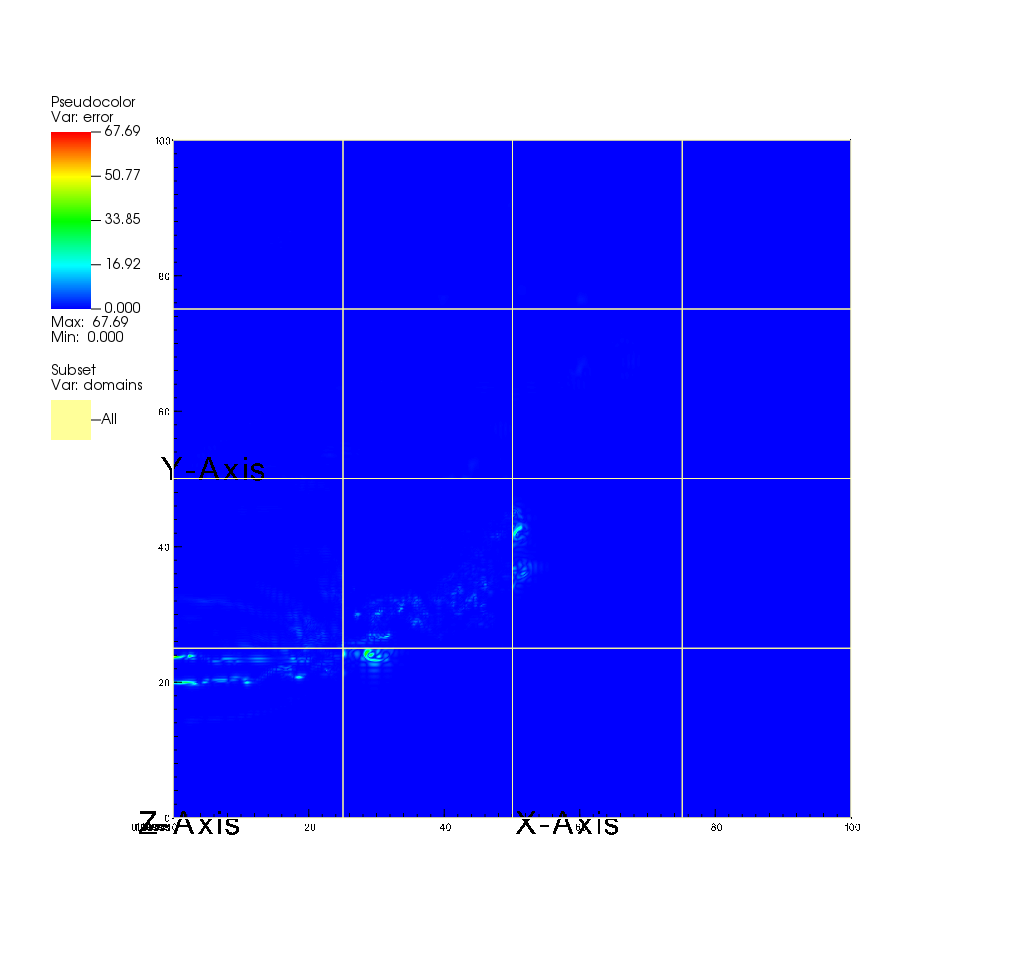
\includegraphics[width=0.44\textwidth]{figures/s3d-error-iter4}}
%	\caption{\comment{2-D slice of the S3D dataset: profile and adaptive error resolution with tolerance=$10^{-2}$}}
%	\label{fig:s3d-adaptive-2d}
%\end{figure}

%The errors in the decoupled LSQ solve shown in \fig{fig:s3d-adaptive-2d-b} has relatively larger errors in the subdomains with strong gradient changes. When including knot adaptivity combined with RAS iterative scheme, the errors in the reconstructed MFA data are reduced to within user-specified relative tolerances of $10^{-2}$. This result demonstrates the convergence of the proposed scheme to adaptively resolve a complex scientific solution profile, even on a small number of subdomains ($\mathcal{N}=16$). 

%\Remark{show error convergence plots for S3D on 16 subdomains with adaptivity}

%that even with the coarse resolution with 16 subdomains, 

%\subsubsection{Nek5000 dataset}
%
%\Remark{add table of actual compression and error as $n_s$ is changed}

%\Remark{Discuss about complications and potential ways to enforce continuity. (a) Use decoded data, (b) Use control point space across interface}



\subsubsection{Parallel Scalability}\label{sec:parallel-scalability}

To demonstrate the parallel performance of the implemented RAS iterative scheme for MFA computation with continuity preservation, we employed both closed-form synthetic and real simulation datasets in \dimension{2} and \dimension{3}. In the following sections, we present both strong scaling and weak scaling studies performed on the Theta Cray XC40 supercomputer operated by the Argonne Leadership Computing Facility (ALCF), which provides 4,392 KNL compute nodes with 64 compute cores and 192 GB DDR4 RAM per node. The interconnect is based on the Aries Dragonfly high speed network.

\subsubsection*{Strong Scaling}

We consider both \dimension{2} and \dimension{3} problems to demonstrate the scaling behavior of the presented parallel MFA computational algorithm in \algo{alg:pseudocode}. One key consideration that drove selection of the subdomain sizes, and the floating knot span descriptions, is motivated by the metric to recover the original error profile from a single subdomain case. 
Verification studies were performed during this strong scaling test to ensure that the local subdomain errors computed on a single task, and on different process counts remain the same at convergence. This verification is important to reiterate the fact that the approximation error due to the constrained solves to recover higher-order continuity does not significantly affect the error metrics for the MFA as $\mathcal{N}$ increases. For this reason, we used synthetic datasets generated with closed form equations for \dimension{2} and \dimension{3} studies as shown in \eqt{eqt:2d-synthetic} and \eqt{eqt:3d-synthetic}.

%The parallel scalability of the implemented RAS iterative solver for ensuring continuity across block boundaries was measured on the 2-D CESM dataset, whose solution profile in a uniform latitude-longitude grid is shown in \fig{fig:cesm-2d-profile}. 
%Our experiments were executed on the Bebop cluster at
%Argonne National Laboratory LCRC (Laboratory Computing Resource Center). Bebop has 1024 public nodes, with Intel Broadwell or Intel Knights Landing processors, with 128 GB memory per Broadwell node, and 104 GB per KNL node. It has an Omni-Path Fabric Interconnect. Broadwell processors have 36 cores, while KNL processors have 64 cores. We primarily used the KNL processors for the scalability tests presented below. \comment{Actually we used haswell nodes here}. 

%\comment{Also mention that the scaling results below were run on Theta ALCF on KNL nodes}

The strong scaling tests were performed on 1 to 16,384 parallel tasks in \dimension{2}, increasing by a factor of $2^2=4$, and the \dimension{3} tests were executed on 1 to 32,768 tasks, increasing by a factor of $2^3=8$. We also note that the \dimension{2} and \dimension{3} case for these studies used 400M and 1.331B input points respectively, with a corresponding $\eta=4$ and $\eta=8$ that was maintained constant for all runs. In order to also better understand the effects of using augmented overlap regions ($\delta$) on scalability, two cases with the choice of $\left| \delta \right|=0$ and $\left| \delta \right|=p$ are shown in \fig{fig:strong-scaling}. 
%
%A strong scalability test was performed on the Bebop cluster with the CESM dataset, using 32 subdomains in the X-direction and 128 subdomains in the Y-direction. With this fixed DD and a uniformly placed, 100 control points per subdomain (10x10) resolution, parallel jobs were executed to compute the MFA. 
%
The Python driver utilized \texttt{DIY} to handle block decompositions and rank assignments, as the total number of tasks used in the parallel run was increased. We measured the overall computational time for setting up the problem, the initial subdomain solves, and the consequent RAS iteration cycle to convergence, which includes the nearest neighbor communication at each iteration. We also show the time for decoding the MFA that is used to measure the errors in each subdomain, and the overall total that includes the effort spent on each of these various tasks. This task-wise breakdown helps us clearly visualize the steps that scale linearly and the ones that do not.

%The time to compute the MFA in parallel is shown for this strong scalability experiment in \fig{fig:cesm-strong-scalability}.

%\begin{figure}[htbp]
%	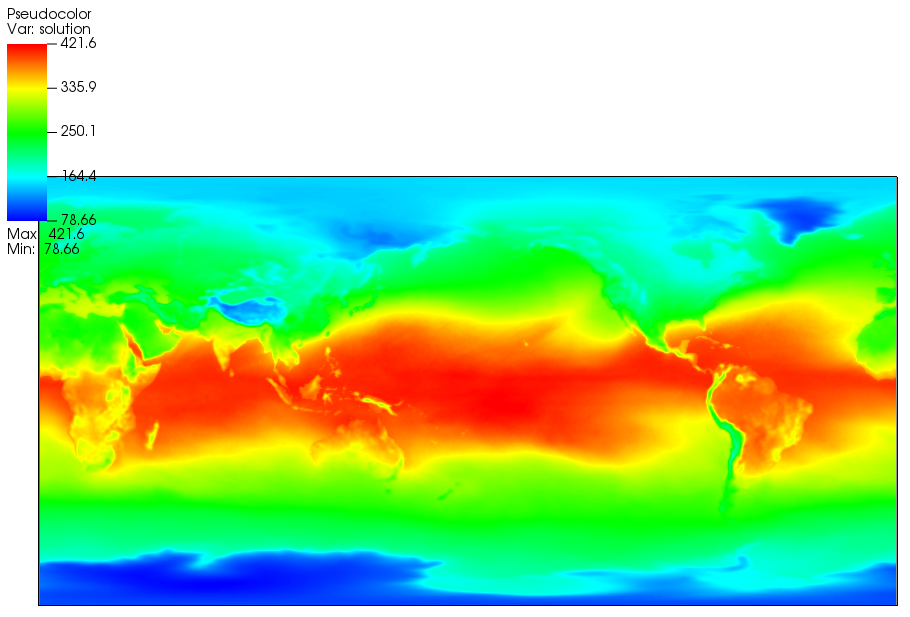
\includegraphics[width=0.45\textwidth]{figures/cesm-profile.png}
%	\caption{2-D CESM climate dataset}
%	\label{fig:cesm-2d-profile}
%\end{figure}



\begin{figure}[htbp]
	\centering
	\subfloat[\dimension{2} strong scaling\label{fig:strong-scaling-2d-a}]{%
		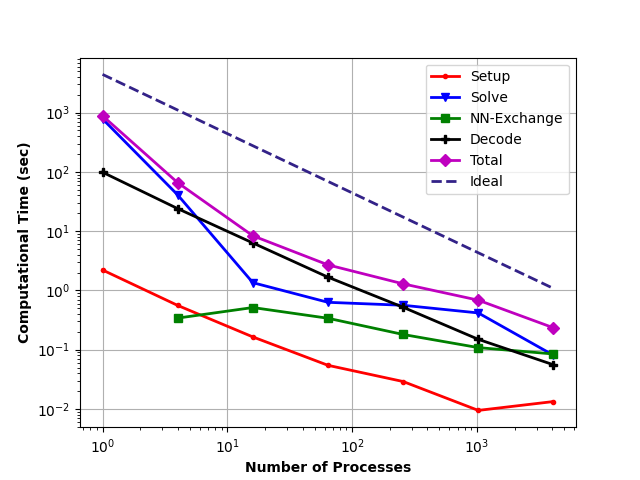
\includegraphics[width=0.49\textwidth]{figures/2d-strong-scaling.png}}
	\subfloat[\dimension{2} strong scaling with $\left| \delta \right|=p$\label{fig:strong-scaling-2d-b}]{%
		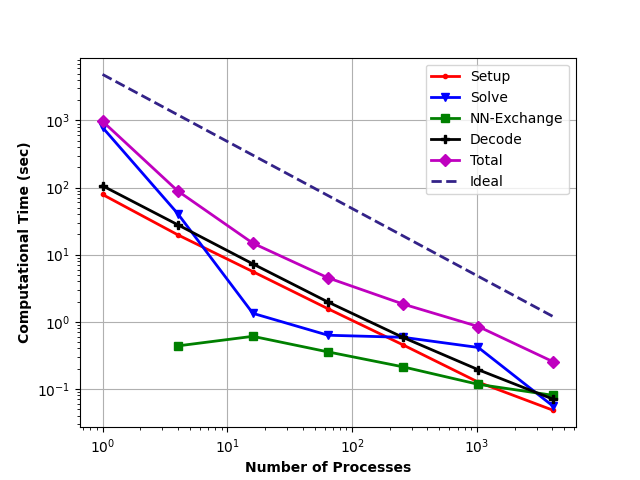
\includegraphics[width=0.49\textwidth]{figures/2d-strong-scaling-aug.png}}\\
	\subfloat[\dimension{3} strong scaling\label{fig:strong-scaling-3d-a}]{%
		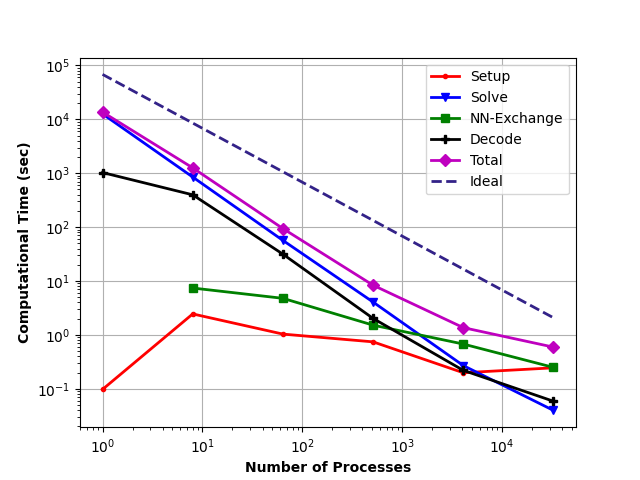
\includegraphics[width=0.49\textwidth]{figures/3d-strong-scaling.png}}
	\subfloat[\dimension{3} strong scaling with $\left| \delta \right|=p$\label{fig:strong-scaling-3d-b}]{%
		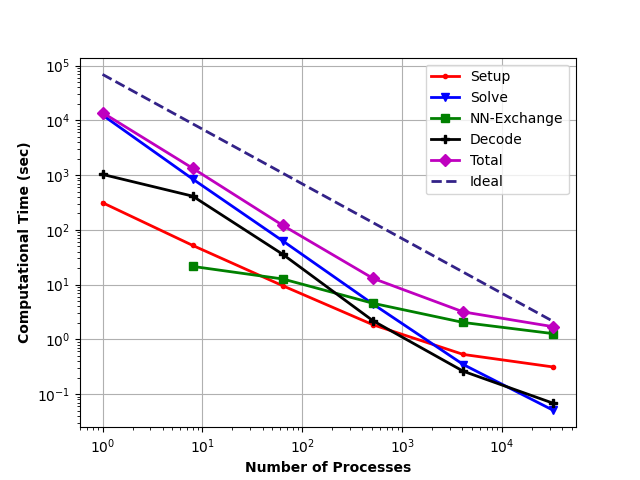
\includegraphics[width=0.49\textwidth]{figures/3d-strong-scaling-aug.png}}\\
	\caption{Strong scaling performance of RAS solver with $p=3$}
	\label{fig:strong-scaling}
\end{figure}


As expected, the RAS iterative scheme shows excellent scalability for the chosen datasets, and the overall time to compute the MFA in parallel was reduced at a nearly ideal rate up to $10^3$ MPI tasks as $\mathcal{N}$ increases, while ensuring $C^{p-1}$ continuity in the subdomain interfaces.  It is important to note that the dominant computational time is driven by the decoupled LSQ solution computation and decoding operations, which are embarassingly parallel as the size of the subdomains (determined by number of knot spans) decreases in direct proportion to the tasks. Given that the scalability of the linear algebraic LSQ solvers \cite{benzi2002, dalcin2011} and Sparse Matrix Vector (SpMV) products used in the decode tasks are well understood, the bottlenecks potentially occur only from the nearest neighbor communication for constraint data exchanges, which remain relatively small in magnitude up to 32K processes tested in the \dimension{3} experiments. The overall strong scaling efficiency remains above 90\% for both overlapping and non-overlapping \dimension{2} problem cases. However, the added setup cost and less than ideally scaling nearest neighbor communications reduce the \dimension{3} problem efficiency for the overlapping subdomain cases to 25\% at 32,768 tasks from 70\% in the nonoverlapping cases. 

Additionally, the parallel efficiency degradation behavior in augmented runs due to the high setup cost occurs due to the current choice of implementations to determine intervals in both the input space data ($\vec{Q}$) and extra knot spans ($\delta$) that need to be exchanged with neighboring subdomains. This setup cost is purely local in the case when $\left| \delta \right|=0$, in contrast to the communication dominated setup when $\left| \delta \right| > 0$. 
%\comment{talk about parallel efficiency values}
It is evident that the cost of nearest neighbor exchanges at scale is driven by the size of the messages being transferred between subdomains, which is a function of $\left| \delta \right|$. The increased amount of data shows smaller degradation in communication for \dimension{2} problems as compared to \dimension{3}, and hence the strong scaling behavior is dependent on the dimension of the problem being solved that is representative of performance in all structured grid solvers for PDEs.

%The ratio of computational work in local subdomain solves in comparison with communication time in nearest-neighbor exchanges gradually increases as subdomain size shrinks. This is due to the fact that global information on smaller subdomains take multiple iterations to propagate, and hence using overlaps for such large problems would be a recommended extension in the future to improve overall scalability of the algorithm. For this intermediate size problem, the strong scaling efficiency of the presented scheme is around 35\% on 2,048 processes, which dropped off from 65\% parallel efficiency at 256 processes.


%\Remark{should we try to do a performance model for this particular case ?
%	communication: C = 4096*4 = 16384 messages
%	serial = 5C + 5A
%	parallel = 5C + 5A/p
%}

%CESM dataset has 6.5M data points
%We used 32*128 = 4096 subdomains for the strong scaling test
%\Remark{How does the nearest neighbor communication stay bounded ? measure timings separately ?}

%jobrun_neup cesm_p1 1 1 python ../Projection-2D.py -x 32 -y 128 -p 5 -c 10 -a 5 --disableadaptivity 

%\begin{figure}
%	\begin{tikzpicture}
%	
%	\begin{loglogaxis}[
%	legend pos= north east,
%%	ymin = 0.0005, ymax = 0.01,
%	xlabel=Number of Processes,
%	ylabel=Time to Compute MFA (secs),
%%	nodes near coords*={\Label},
%%	visualization depends on={value \thisrow{label} \as \Label},
%	grid=both,
%	grid style={line width=.1pt, draw=gray!10},
%	major grid style={line width=.2pt,draw=gray!50},
%	axis line style={latex-latex},
%	every axis plot/.append style={line width=1.0pt},
%	%axis lines=middle,
%	]
%	\axispath\draw
%	(7.49165,-10.02171)
%	|-  (8.31801,-11.32467)
%	node[near start,left] {$\frac{dy}{dx} = -2.58$};
%	
%	\addplot[smooth,mark=*,blue,width=5pt] table [meta=eff]  {
%		x y eff
%		1	7045.451504	100
%		2	4137.296798	85.14558959
%		4	2322.884537	75.82653583
%		8	1061.974002	82.92871918
%		16	544.925238	80.80754722
%		32	314.578249	69.98906001
%		64	150.8316872	72.98544611
%		128	83.16858159	66.18195096
%		256	42.09792775	65.37446476
%		512	25.07828297	54.870772
%		1024	17.07229925	40.30109616
%		2048	9.898160849	34.75556641
%%		4096	8.519652482	20.18956686
%	};
%
%	\addplot[dashed,black,width=2pt] table [meta=class]  {
%	x y class 
%	1	40000	100
%	2	20000	100
%	4	10000	100
%	8	5000	100
%	16	2500	100
%	32	1250	100
%	64	625	100
%	128	312.5	100
%	256	156.25	100
%	512	78.125	100
%	1024	39.0625	100
%	2048	19.53125	100
%%	4096	9.765625	100
%};
%	
%	\legend{Scalability\\Ideal\\}
%	
%	\end{loglogaxis}
%	\end{tikzpicture}
%	\caption{Strong scalability of the 2-D CESM Problem with 4,096 subdomains and 100 control points/subdomain}
%	\label{fig:cesm-strong-scalability}
%\end{figure}




\subsubsection*{Weak Scaling}

Given that the performance of the overlapping and augmented MFA scheme was comparable to non-overlapping cases ($\left| \delta \right|=0$), and since the error reduction from having extra overlaps always results in better solution recovery, we strictly focus on overlapping cases alone for the weak scaling study. Here, the overall work per subdomain is maintained constant, and the number of tasks are increased from 1 to 16,384 in \dimension{2}, and from 1 to 32,768 in \dimension{3}, similar to the strong scaling study.
The weak scaling results maintaining an overall MFA compression rate of $\eta=2^d,\forall d \in [2,3]$ is shown in \fig{fig:weak-scaling}.


\begin{figure}[htbp]
	\centering
	\subfloat[\dimension{2} weak scaling\label{fig:weak-scaling-2d}]{%
		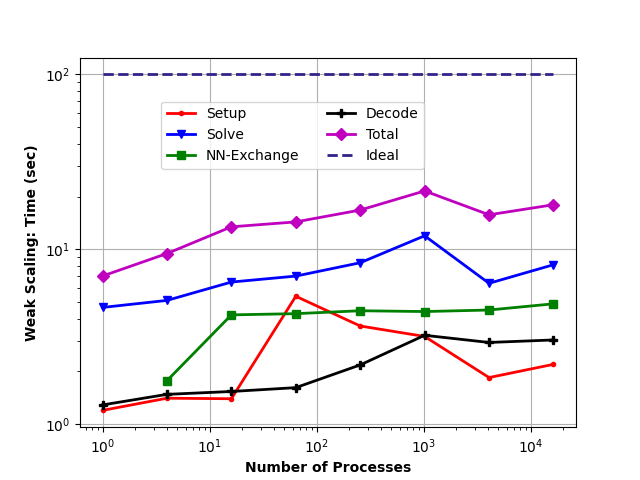
\includegraphics[width=0.5\textwidth]{figures/2d-weak-scaling.png}}
	\hfill
	\subfloat[\dimension{3} weak scaling\label{fig:weak-scaling-3d}]{%
		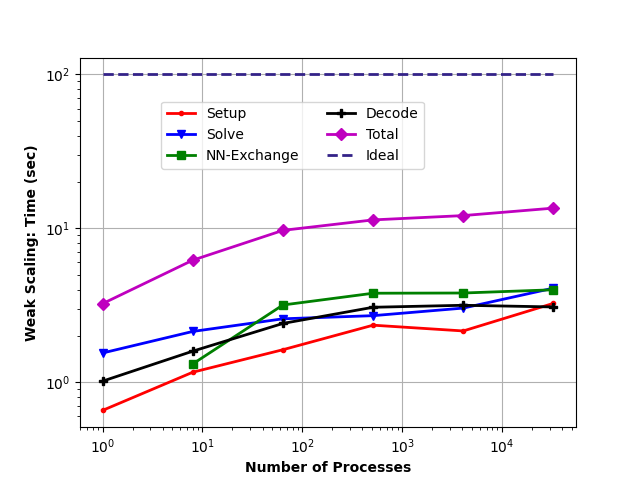
\includegraphics[width=0.5\textwidth]{figures/3d-weak-scaling.png}}\\
	\caption{Weak scaling performance of RAS solver with $p=3$ and $\left| \delta \right|=p$}
	\label{fig:weak-scaling}
\end{figure}

The weak scaling study demonstrates that the overall performance of the RAS iterative scheme for large number of subdomains does not significantly affect the parallel efficiency, which are around 40\% in \dimension{2} and 24\% in \dimension{3} at the fine limit tested. The subdomain solve and nearest neighbor data exchange dominate the overall time to solution. However, it is important to note that the actual runtime for the MFA computation only grows by a factor of 2, even on 16K processes or more. 


\subsubsection*{Performance Study on S3D Dataset}

Finally, we consider the case of the S3D combustion dataset shown in \fig{fig:s3d-ref-error} and measure the strong scaling performance on up to 1024 processes. Using parallel MPI-IO implemented with \texttt{DIY}, and exposed through the Python interface, a strong scaling performance study was measured on this realistic dataset and shown in \fig{fig:s3d-strong-scaling}. Note that the IO cost for reading the chunk of data required on each task is included in the setup time shown in the figure.

The performance and error analysis indicate good speedup to reduce overall time for MFA computation, until nearest neighbor communication and data exchanges start dominating the overall workflow. These results show similar behavior to the strong scaling studies performed on synthetic datasets and provide confirmation on the feasibility of the presented approach for tackling real-world large datasets.

\begin{figure}[htbp]
	\centering
	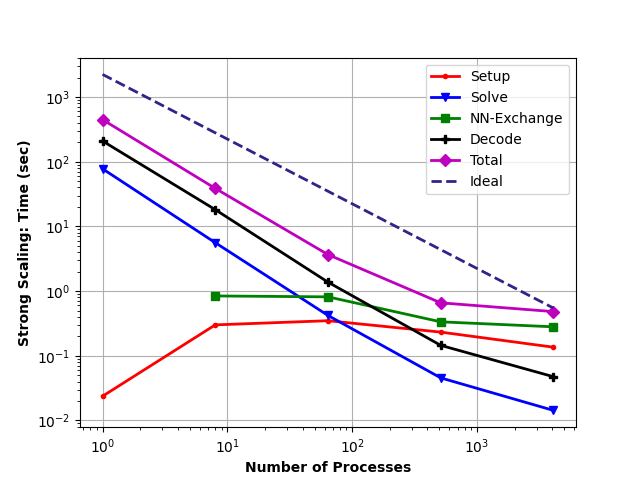
\includegraphics[width=0.6\textwidth]{figures/problem-s3d-strong-scaling.png}
	\caption{Strong scaling for the S3D dataset with $p=5$}
	\label{fig:s3d-strong-scaling}
\end{figure}


%\paragraph{Positioning Figures and Tables} Place figures and tables at the top and 
%``Fig.~\ref{fig}'', even at the beginning of a sentence.

%\begin{table}[htbp]
%\caption{Table Type Styles}
%\begin{center}
%\begin{tabular}{|c|c|c|c|}
%\hline
%\textbf{Table}&\multicolumn{3}{|c|}{\textbf{Table Column Head}} \\
%\cline{2-4} 
%\textbf{Head} & \textbf{\textit{Table column subhead}}& \textbf{\textit{Subhead}}& \textbf{\textit{Subhead}} \\
%\hline
%copy& More table copy$^{\mathrm{a}}$& &  \\
%\hline
%\multicolumn{4}{l}{$^{\mathrm{a}}$Sample of a Table footnote.}
%\end{tabular}
%\label{tab1}
%\end{center}
%\end{table}

%\begin{figure}[htbp]
%\centerline{\includegraphics{fig1.png}}
%\caption{Example of a figure caption.}
%\label{fig}
%\end{figure}
